\documentclass[11pt]{article}
\usepackage[T1]{fontenc}
\usepackage[utf8]{inputenc}
\usepackage{lmodern}
\usepackage{amsmath,amssymb,amsthm,mathtools}
\usepackage[margin=1in]{geometry}
\usepackage{microtype,booktabs,array,enumitem}
\usepackage{xcolor,tikz}
\usetikzlibrary{arrows.meta,positioning,calc,decorations.pathreplacing}
\definecolor{linkblue}{rgb}{0.05,0.18,0.32}
\usepackage[colorlinks=true,linkcolor=linkblue,citecolor=linkblue,urlcolor=linkblue]{hyperref}
\hypersetup{pdftitle={Sharp Logarithmic Exponents for Fixed Off-Diagonal Ramsey Numbers},
  pdfauthor={OpenAI},bookmarksdepth=2}
\numberwithin{equation}{section}
\newtheorem{theorem}{Theorem}[section]
\newtheorem{lemma}[theorem]{Lemma}
\newtheorem{proposition}[theorem]{Proposition}
\newtheorem{corollary}[theorem]{Corollary}
\theoremstyle{definition}
\newtheorem{definition}[theorem]{Definition}
\theoremstyle{remark}
\newtheorem{remark}[theorem]{Remark}
\newcommand{\F}{\mathbb F}
\newcommand{\E}{\mathbb E}
\newcommand{\Prob}{\mathbb P}
\DeclareMathOperator{\PG}{PG}
\DeclareMathOperator{\KL}{KL}
\DeclareMathOperator{\TV}{TV}
\DeclareMathOperator{\Span}{span}
\DeclareMathOperator{\supp}{supp}
\setlist{itemsep=3pt,topsep=5pt}
\setcounter{tocdepth}{1}
\title{Sharp Logarithmic Exponents for Fixed\newline Off-Diagonal Ramsey Numbers}
\author{OpenAI}
\date{September 24, 2026}
\begin{document}
\maketitle
\begin{abstract}
For every fixed integer $s\ge6$, we determine the sharp logarithmic exponent
of the off-diagonal Ramsey number:
\[
 r(s,t)=\frac{t^{s-1}}{(\log t)^{s-2+o(1)}}
 \qquad (t\longrightarrow\infty).
\]
\end{abstract}
\tableofcontents
\clearpage
\section{Introduction}
\label{intro:section}

For integers $s,t\ge2$, the Ramsey number $r(s,t)$ is the least integer
$N$ such that every finite simple graph on $N$ vertices contains a clique
of order $s$ or an independent set of order $t$. We study the
off-diagonal regime in which $s$ is fixed and $t$ tends to infinity
through the integers. All logarithms are natural.

\begin{theorem}\label{intro:main}
For every fixed integer $s\ge6$ there is a constant $C_s>0$ such that,
for every $\varepsilon>0$ and every sufficiently large integer $t$,
\[
 \frac{t^{s-1}}{(\log t)^{s-2+\varepsilon}}
 \le r(s,t)
 \le C_s\frac{t^{s-1}}{(\log t)^{s-2}}.
\]
In particular,
\[
 \lim_{t\to\infty}
 \frac{(s-1)\log t-\log r(s,t)}{\log\log t}=s-2.
\]
\end{theorem}

The theorem determines the logarithmic exponent. It does not assert
that $r(s,t)$ is bounded below by a positive constant times
$t^{s-1}/(\log t)^{s-2}$.

\subsection{Background and contribution}

Ramsey's finite partition theorem, developed in his work on a problem
of formal logic, guarantees that these numbers are finite
\cite[Theorem~B]{Ramsey1930}.
The classical argument of Erd\H{o}s and Szekeres gives
\[
 r(s,t)\le\binom{s+t-2}{s-1}
\]
and hence the polynomial upper bound $O_s(t^{s-1})$
\cite{ErdosSzekeres1935}. Ajtai, Koml\'os, and Szemer\'edi obtained the
logarithmic improvement
$O_s(t^{s-1}/(\log t)^{s-2})$ \cite{AKS1980}.
Li, Rousseau, and Zang subsequently proved the upper estimate with
leading coefficient $1+o(1)$ \cite{LiRousseauZang2001}.
The logarithmic power $s-2$ thus comes from the classical upper-bound
side of the problem. Determining whether a lower construction attains
that power requires controlling independent sets far more precisely
than the polynomial exponent alone.

For $s=3$, Kim's lower bound established
$r(3,t)=\Theta(t^2/\log t)$ \cite{Kim1995}.
For fixed $s\ge5$, Spencer's local-lemma construction gives
$r(s,t)=\Omega_s((t/\log t)^{(s+1)/2})$ \cite{Spencer1977}.
Bohman and Keevash improved the logarithmic factor through the random
$K_s$-free process, proving
\[
 r(s,t)=\Omega_s\!\left(
 t^{(s+1)/2}(\log t)^{1/(s-2)-(s+1)/2}\right)
\]
\cite[Theorem~1.2]{BohmanKeevash2010}.
A different route uses finite geometry and pseudorandom graphs.
Mubayi and Verstra\"ete showed that suitable density-optimal
$K_s$-free pseudorandom graphs would yield the lower order
$t^{s-1}/(\log t)^{2s-4}$ \cite[Corollary~2]{MubayiVerstraete2024}; this is a
conditional construction criterion.
For $s=4$, Mattheus and Verstra\"ete obtained the unconditional bound
$\Omega(t^3/(\log t)^4)$ using a finite-geometric construction
\cite{MattheusVerstraete2024}.
Brada\v{c}'s projective construction then established
\[
 r(s,t)\ge c_s\frac{t^{s-1}}{(\log t)^{2s-4}}
 \qquad(s\ge3,\ t\ge2)
\]
\cite[Theorem~1.1]{Bradac2026}, determining the polynomial exponent
for every fixed $s$. The remaining difference between the powers
$2s-4$ and $s-2$ is the logarithmic gap addressed here.

The geometric ingredients also have an earlier history.
Projective orthogonality and its spectral estimates appear in
Alon and Krivelevich \cite{AlonKrivelevich1997}.
Ordered incidence constructions of Codenotti, Pudl\'ak, and Resta
\cite{CodenottiPudlakResta2000}, and Kostochka, Pudl\'ak, and R\"odl
\cite{KostochkaPudlakRodl2010}, are predecessors of the flag approach.
We use the ordered incident-flag graph of Brada\v{c}'s
higher-dimensional construction \cite[Section~2.5]{Bradac2026}
and adapt its marking argument \cite[Claim~2.13]{Bradac2026}.
The distinction between a step that substantially shrinks a candidate
set and a step with few possible choices also appears in the
independent-set counting argument of Alon and R\"odl
\cite[proof of Theorem~2.1]{AlonRodl2005}. Here it must be combined with an entropy estimate
for a sequence selected from the random stream: selection need not
preserve the independence or uniformity of its flags.

The companion paper \emph{The sharp logarithmic exponent of $r(5,t)$}
\cite[Lemma~3.4 and Theorem~4.1]{RamseyFive} develops the selected-law entropy and
low-dimensional sparse-pair framework for $s=5$.
The present paper supplies all the required arguments locally.
To pass to arbitrary fixed dimension, we prove a repeated-projection
reduction for sparse pairs and a two-row high-rank description using
a rich-subspace bound that follows from Nie and Wang's finite-degree
closure inequality \cite{NieWang2015}.
The repeated projections and the high-rank construction require their
own estimates; neither is inferred from the five-clique theorem.
The low-dimensional polynomial argument adapts methods of Dvir,
Guth--Katz, and Elekes--Kaplan--Sharir
\cite{Dvir2009,GuthKatz2010,ElekesKaplanSharir2011}, with the
positive-characteristic obstructions analyzed by Ellenberg and
Hablicsek explicitly controlled \cite{EllenbergHablicsek2016}.

\subsection{The construction and its entropy obstruction}

The main work is the following prime-indexed construction. For a graph
$G$, write $\alpha(G)$ for its independence number.

\begin{theorem}\label{intro:prime-construction}
Fix an integer $d\ge5$ and a real number $0<\eta<1/10$.
For every sufficiently large prime $q$, with $\sigma=\log q$, there is
a graph $G$ such that
\[
 |V(G)|=\lfloor q^d\sigma\rfloor,\qquad
 K_{d+1}\not\subseteq G,\qquad
 \alpha(G)<\lfloor q\sigma^{1+\eta}\rfloor.
\]
\end{theorem}

Here is the construction and the organization of its proof. A point of
$\PG(d,q)$ is a one-dimensional vector subspace of $\F_q^{d+1}$.
A dual point is a one-dimensional subspace of the dual vector space;
it specifies a projective hyperplane. Write $a\perp b$ when the
covector $b$ vanishes on the point $a$. An incident flag is a pair
$(a,b)$ with $a\perp b$.

Choose $N=\lfloor q^d\sigma\rfloor$ flags independently and uniformly,
and use their positions as vertices. Positions $i<j$ are adjacent when
\[
 a_i\perp b_j\quad\hbox{and}\quad a_j\not\perp b_i.
\]
Linear independence excludes $K_{d+1}$. An independent set, in its
original order, is therefore a flag sequence satisfying
\[
 i<j,\quad a_i\perp b_j\quad\Longrightarrow\quad a_j\perp b_i.
\]
We call this condition consistency. Its asymmetry records the order;
reversing the order and interchanging the two endpoint spaces preserves
the condition.

Suppose that every stream of flags contained a consistent sequence of
length $k=\lfloor q\sigma^{1+\eta}\rfloor$. Selecting such a sequence
can heavily bias its distribution. Nevertheless, a counting argument
gives every selected sequence $F$ of deterministic length
$\ell=\Theta(k)$ the entropy lower bound
\[
 H(F)\ge d\sigma\ell+\eta\ell\log\sigma-O(k).
\]
This bound survives any fixed number of restrictions to events of
probability bounded below. We will contradict it by successively
describing shorter sequences, still of length $\Theta(k)$, in smaller
flag domains.

The cost of the exceptional positions in the marking argument explains
why these successive descriptions are needed. Brada\v{c}'s direct count
records $O(q\sigma)$ expensive flags, with $O(\sigma)$ information
per flag \cite[proof of Lemma~2.12]{Bradac2026}. The resulting
$O(q\sigma^2)$ allowance is too coarse for the present entropy
comparison: its scale exceeds the surplus $\eta\ell\log\sigma$ when
$\ell=\Theta(q\sigma^{1+\eta})$. The leading term $d\sigma\ell$
already allows $d\sigma$ units for each retained flag. Smaller flag
domains reduce the excess cost of the expensive positions beyond this
allowance. At each stage we replace the old description instead of
carrying its history into the new message.

The description has three main components.

\paragraph{Describing a sparse pair of point sets.}
Given point sets $S,T$ in opposite point systems of $\PG(j,q)$, where
$2\le j\le d$, assume that
$|S||T|$ is close on a logarithmic scale to $q^{j+1}$, while their
incidence density is much smaller than $1/q$. The geometric description
lemma produces a short message specifying a set that captures a fixed
fraction of the smaller support and is not much larger than that
support. Separate validation samples then produce small domains on
both sides that retain almost all of $S$ and $T$.
Sections~\ref{geom:section} and~\ref{learn:section} prove this statement.
Repeated projection reduces dimensions $j\ge4$ to dimensions two and
three. In the remaining dimensions, the sampling argument uses independent
Poisson batches. A moment argument controls the size of the decoded set;
its geometric input is a rich-line estimate with the field characteristic
kept larger than the relevant polynomial degrees.

\paragraph{Finding supports to which the description applies.}
Consistency lets us mark all but $O(q\log q)$ positions as belonging
to explicitly known flag domains of size $O(q^d)$. The entropy deficit
in these domains bounds the dependence between suitable representative
positions and the remaining sequence. Most representative pairs
therefore have almost no one-way incidence conflict. In the reciprocal
classes, whose two prescribed endpoint-domain bounds have product
$O(q^{d+1})$, a geometric argument turns this into sparse incidence
between endpoint supports. Possible exact
incidence coincidences are charged to small occupied flag rectangles.
Section~\ref{mark:section} supplies these estimates. The other classes
have large endpoint ranks; Section~\ref{comp:section} describes them
directly using two independent sample rows and a polynomial bound for
the union of rich subspaces.

\paragraph{Iterating without retaining old information.}
For reciprocal supports, arrange the representative pairs in time
order and apply the geometric description along a balanced binary
tree. Each successful node restricts one endpoint domain for each
child. Fresh validation samples bound the loss from each restriction
before any later success is imposed. An additive potential bounds the
total message length. Crucially, the new decoder starts with the full
projective spaces and reads only the new message: it does not need the
previous context, hidden supports, or their conditional laws.
Section~\ref{comp:section} proves this one-step improvement, and
Section~\ref{end:section} iterates it a bounded number of times. The
resulting entropy upper bound is $d\sigma\ell+O(k)$, contradicting the
displayed lower bound.

The tables used to select description samples are public auxiliary
randomness. We bound message length, not search time. After averaging
over these tables, they can be fixed before imposing the next
constant-probability restriction on the stream.

Section~\ref{base:section} establishes the projective and information
estimates used throughout. The final section also transfers
Theorem~\ref{intro:prime-construction} from prime parameters to all
sufficiently large integers $t$ and proves the upper bound in
Theorem~\ref{intro:main}.

\section{Flags, incidence, and selected-tuple entropy}
\label{base:section}

Fix an integer $d\ge5$ and $0<\eta<1/10$. Throughout the construction,
$q$ is a sufficiently large prime, and
\begin{equation}
 \sigma=\log q,\qquad N=\lfloor q^d\sigma\rfloor,
 \qquad k=\lfloor q\sigma^{1+\eta}\rfloor.
 \label{base:stream-parameters}
\end{equation}
Constants may depend on $d,\eta$ and on fixed retention and budget
constants, but not on $q$. In particular, the constants implicit in
$\ell=\Theta(k)$ do not change with $q$.
We first construct a graph that always excludes $K_{d+1}$. The remaining
task will be to exclude a consistent $k$-tuple of its flags. The entropy
bound below identifies the amount of information that any selected tuple
must retain, even when its selection is highly biased.

\subsection{Projective incidence}

The following point--hyperplane calculation is the bipartite form of the
projective orthogonality estimate used by Alon and Krivelevich
\cite{AlonKrivelevich1997}; we include the weighted identity needed later.

For $j\ge1$, let $V_j=\F_q^{j+1}$ and let $V_j^*$ be its dual vector
space. The two projective spaces $\PG(V_j)$ and $\PG(V_j^*)$ consist of
one-dimensional vector subspaces; both have size
\[
 Q_j=1+q+\cdots+q^j.
\]
Set $Q_0=1$. A point $a\in\PG(V_j)$ and a dual point
$b\in\PG(V_j^*)$ are incident, written $a\perp b$, if every covector
in $b$ vanishes on $a$. Thus a dual point also represents a hyperplane
in $\PG(V_j)$. All dimensions of linear spans below are \emph{vector}
dimensions; a vector subspace of dimension $r\ge1$ has $Q_{r-1}$
projective points. For sets in the opposite projective spaces, write
$e(S,T)$ for their number of incident pairs.

\begin{lemma}[Weighted incidence estimates]
\label{base:incidence}
Let $j\ge2$, and put $p_j=Q_{j-1}/Q_j=(1-Q_j^{-1})/q$.
For any real weights $w_x$ on one of the two projective spaces,
\begin{equation}
 \sum_y\left(\sum_{x\perp y}w_x-p_j\sum_xw_x\right)^2
 =q^{j-1}\left(\sum_xw_x^2-\frac{(\sum_xw_x)^2}{Q_j}\right)
 \le q^{j-1}\sum_xw_x^2.
 \label{base:weighted-variance}
\end{equation}
In particular, for sets $S,T$ in the opposite spaces,
\begin{equation}
 \left|e(S,T)-p_j|S||T|\right|
 \le q^{(j-1)/2}\sqrt{|S||T|}.
 \label{base:mixing}
\end{equation}
If $S,T$ are nonempty and $e(S,T)/(|S||T|)=o(1/q)$, then
$|S||T|\le Cq^{j+1}$ for all sufficiently large $q$.
\end{lemma}

\begin{proof}
Let $M$ be the point-hyperplane incidence matrix. Every point lies in
$Q_{j-1}$ hyperplanes, and two distinct points lie in $Q_{j-2}$
hyperplanes. Hence, writing $J$ for the all-ones matrix,
\[
 MM^{\mathsf T}=q^{j-1}I+Q_{j-2}J.
\]
The same identity holds with the two projective spaces interchanged.
Subtract the mean of $w$ and apply this identity to obtain
Equation~\eqref{base:weighted-variance}. Applying the resulting operator
norm bound to the centered indicators of $S$ and $T$ proves
Equation~\eqref{base:mixing}. Finally, $p_j=(1+o(1))/q$, so the sparsity
assumption and Equation~\eqref{base:mixing} give
\[
 \frac{|S||T|}{2q}
 \le q^{(j-1)/2}\sqrt{|S||T|}
\]
for large $q$, proving the last assertion.
\end{proof}

\subsection{The flag graph and rectangles}

We use Brada\v{c}'s ordered flag construction
\cite[Section~2.5]{Bradac2026}. A \emph{flag} in dimension $d$ is an incident pair $(a,b)$ in
$\PG(V_d)\times\PG(V_d^*)$. There are $Q_dQ_{d-1}$ flags. Sample an
ordered stream of $N$ independent uniform flags $(a_i,b_i)$, and make
a graph on its positions $1,\ldots,N$ by declaring, for $i<j$,
\begin{equation}
 ij\in E(G)\quad\Longleftrightarrow\quad
 a_i\perp b_j\ \hbox{ and }\ a_j\not\perp b_i.
 \label{base:edge-rule}
\end{equation}
Repeated flags are allowed: graph vertices are positions, not flag
values. An ordered flag tuple is called \emph{consistent} if
\begin{equation}
 i<j,\quad a_i\perp b_j\quad\Longrightarrow\quad a_j\perp b_i.
 \label{base:consistency}
\end{equation}

\begin{lemma}[Flag graph]
\label{base:flag-graph}
Every graph defined by Equation~\eqref{base:edge-rule} is $K_{d+1}$-free.
Its independent sets, in increasing position order, are exactly its
consistent subtuples. Reversing a consistent tuple and interchanging
its first and second endpoints preserves consistency.
\end{lemma}

\begin{proof}
Consider a clique with flags $(a_1,b_1),\ldots,(a_m,b_m)$ in its
increasing position order. For $r<m$, the covector $b_r$ annihilates
$a_1,\ldots,a_r$ but not $a_{r+1}$. The first assertion follows from
the earlier clique edges and the flag condition; the second follows
from the edge between positions $r$ and $r+1$. Thus $a_{r+1}$ lies
outside the vector span of its predecessors. The $m$ lines are
independent, while the nonzero covector $b_m$ annihilates all of them.
Its kernel has dimension $d$, so $m\le d$.
Negating Equation~\eqref{base:edge-rule} gives
Equation~\eqref{base:consistency}. Reversal and dual interchange turn
that same implication into itself.
\end{proof}

For a vector subspace $U\subseteq V_d^*$, define the rectangle
\[
 \mathcal R(U)=
 \{(a,b):b\subseteq U,\ a\subseteq U^\perp\}.
\]
All pairs in this set are flags. The next estimate holds simultaneously
for every rectangle, including a rectangle chosen from previously
observed data.

\begin{lemma}[Simultaneous rectangle occupancy]
\label{base:rectangles}
There is a constant $C_d$ such that, with probability $1-o(1)$, every
$\mathcal R(U)$ contains at most $C_d\sigma$ positions of the uniform
stream. The same event controls rectangles after dual interchange.
\end{lemma}

\begin{proof}
If $\dim U=r$ with $1\le r\le d$, then
\[
 |\mathcal R(U)|=Q_{r-1}Q_{d-r}\le4q^{d-1}.
\]
The rectangles for $r=0,d+1$ are empty. Thus the occupancy of any
fixed rectangle is binomial with mean at most $4\sigma$. There are
at most $(d+2)q^{(d+1)^2}$ subspaces, by counting possible ordered
bases. For $A>4e$, the exponential-moment bound for a binomial variable
gives
\[
 \Prob\{\text{occupancy}>A\sigma\}
 \le (4e/A)^{A\sigma}
 =q^{-A\log(A/(4e))},
\]
with an immaterial adjustment for rounding the threshold. Choose $A$
large enough in terms of $d$ and sum over the subspaces. Under dual
interchange, $\mathcal R(U)$ becomes the rectangle defined by
$U^\perp$, so no further event is needed.
\end{proof}

\subsection{Entropy after arbitrary selection}

For a discrete random variable $X$ with mass function $p$, write
$H(X)=-\sum_xp(x)\log p(x)$, with $0\log0=0$. Entropies use natural
units. Conditional entropy is the average of the corresponding
conditional entropies. Expanding these sums gives the chain rule and
\[
 I(X;Y)=H(X)+H(Y)-H(X,Y)
       =\KL(P_{X,Y}\Vert P_X\otimes P_Y),
\]
where $\KL(P\Vert Q)=\sum_xP(x)\log(P(x)/Q(x))$ is infinite if
$P$ is not absolutely continuous with respect to $Q$. These identities
also apply to countable variables of finite entropy.

\begin{lemma}[Selected-tuple entropy]
\label{base:selection-entropy}
Let a random stream have law dominated by $C_0$ times the iid uniform
flag-stream law, where $C_0$ is independent of $q$. From this stream,
using arbitrary dependent auxiliary randomness, extract a tuple $F$
of deterministic length $\ell=\Theta(k)$. Its order may be either
increasing stream order or reversed stream order with the endpoints
interchanged. Then
\begin{equation}
 H(F)\ge d\sigma\ell+\eta\ell\log\sigma-O(k).
 \label{base:entropy-lower}
\end{equation}
The implicit constant may depend on $C_0$ and the fixed comparison
constants in $\ell=\Theta(k)$.
\end{lemma}

\begin{proof}
For any prescribed tuple $f$, the event $F=f$ implies that $f$ occurs
on some increasing set of $\ell$ stream positions, in one of the two
allowed orientations. For each such set and orientation its iid
probability is $(Q_dQ_{d-1})^{-\ell}$. The stream domination and a
union bound therefore give
\[
 \Prob(F=f)\le2C_0\binom N\ell(Q_dQ_{d-1})^{-\ell}.
\]
This containment of events uses no assumption about the selector's
conditional distribution. Shannon entropy is at least minus the
logarithm of the largest atom. Now
\[
 \log(Q_dQ_{d-1})=(2d-1)\sigma+O(1/q),
 \qquad
 \log(eN/\ell)=(d-1)\sigma-\eta\log\sigma+O(1).
\]
Use $\binom N\ell\le(eN/\ell)^\ell$ and $\ell=\Theta(k)$ to conclude.
\end{proof}

The positive term $\eta\ell\log\sigma$ is the eventual contradiction:
we shall successively describe a selected tuple using only
$d\sigma\ell+O(k)$ entropy. Constant-probability restrictions of the
stream law are compatible with Lemma~\ref{base:selection-entropy}.
Indeed, if the current domination factor is $C_0$ and an event in the
joint probability space has probability at least $c>0$, then after
conditioning the stream marginal is dominated by $C_0/c$ times the
original law. This remains true when that event also uses auxiliary
randomness. A fixed number of such restrictions preserves a constant
domination factor.

\begin{lemma}[Transferring a rare event]
\label{base:event-transfer}
For two probability laws $P,Q$ on the same finite or countable space
and an event $E$,
\begin{equation}
 Q(E)\le\frac{\KL(P\Vert Q)+P(E)}{1-e^{-1}}.
 \label{base:kl-event}
\end{equation}
\end{lemma}

\begin{proof}
The assertion is immediate when the relative entropy is infinite.
Otherwise Jensen's inequality gives, for bounded $f$,
\[
 \KL(P\Vert Q)\ge \E_P f-\log\E_Q e^f.
\]
Apply this with $f=-1_E$. Since $-\log(1-u)\ge u$ for $0\le u<1$,
\[
 \KL(P\Vert Q)
 \ge-P(E)-\log\bigl(1-(1-e^{-1})Q(E)\bigr)
 \ge-P(E)+(1-e^{-1})Q(E),
\]
which proves the claim.
\end{proof}

\begin{lemma}[Elementary sampling tails]
\label{base:tails}
If $X$ is binomial or Poisson with mean $\mu$, then
$\E e^{tX}\le\exp((e^t-1)\mu)$ for every real $t$. For each fixed
$0<\delta<1$ there is $c_\delta>0$ such that
\[
 \Prob(|X-\mu|\ge\delta\mu)\le2e^{-c_\delta\mu}.
\]
For $h\ge e\mu>0$,
\[
 \Prob(X\ge h)\le(e\mu/h)^h.
\]
When $\mu=0$, the variable is zero almost surely.
\end{lemma}

\begin{proof}
For a Bernoulli variable of mean $p$, its exponential moment is
$1+p(e^t-1)\le e^{p(e^t-1)}$; multiply over independent trials.
For a Poisson variable the moment formula is an equality, by summing
its series. Exponential Markov with $t=\log(1+\delta)$ or
$t=\log(1-\delta)$ gives the two proportional tails. For the final
bound use $t=\log(h/\mu)$ and discard the factor $e^{-\mu}$.
\end{proof}

\subsection{The scales of a description}

The geometric descriptions and the compression stages use the following
common scales. Their input is a deterministic number $D$ measuring the
current description budget; the precise budget interpretation will be
given when a compression stage is defined. At present we need only its
allowed interval. Set
\begin{equation}
\begin{gathered}
 \beta=\eta/10^7,\qquad
 \sigma^\beta\le D\le\sigma^{1-\eta/2},\\
 K=D\sigma^{3\beta},\qquad K_*=D\sigma^{6\beta},\qquad
 L=D\sigma^{8\beta},\qquad P=LR,\\
 \sigma^\beta\le R\le2\sigma^\beta+2,
 \qquad R\text{ an even integer chosen deterministically}.
\end{gathered}
\label{base:parameters}
\end{equation}
The choice $R=2\lceil\sigma^\beta/2\rceil$ is one possibility.

\begin{lemma}[Separation of scales]
\label{base:scale-comparisons}
Uniformly over the interval for $D$ in Equation~\eqref{base:parameters},
\[
 K_*=o(L),\qquad L=o(P),\qquad P=o(\sigma),\qquad
 R\log L+\log\sigma=o(P).
\]
Moreover, for sufficiently large $q$,
$D\sigma^{9\beta}\le P\le4D\sigma^{9\beta}$.
\end{lemma}

\begin{proof}
The last bounds follow from the interval for $R$.
Also $K_*/L=\sigma^{-2\beta}$ and $L/P=1/R\le\sigma^{-\beta}$.
Since $9\beta<\eta/2$,
\[
 P\le4\sigma^{1-\eta/2+9\beta}=o(\sigma).
\]
Finally $L\ge\sigma^{9\beta}$, $P\ge\sigma^{10\beta}$, and
$\log L=O(\log\sigma)$, so
\[
 \frac{R\log L}{P}=\frac{\log L}{L}=o(1),
 \qquad \frac{\log\sigma}{P}=o(1).
\]
\end{proof}

\section{Describing sparse pairs: validation and geometry}
\label{geom:section}

We now describe one side of a pair having unusually few incidences. The
decoder knows domains containing the two supports, but not the supports
themselves. The description will give a moderately enlarged set capturing
a fixed fraction of the smaller support. A separate validation step turns
this into almost complete capture on both sides. Dimensions at least four
are reduced by projection; the remaining geometric input concerns lines
and planes in projective dimension three. Section~\ref{learn:section}
supplies the sampling argument that completes the low-dimensional case.

Throughout this section, the parameters are those in
\eqref{base:parameters}; in particular, $q$ is prime and $P=o(\sigma)$,
where $\sigma=\log q$. All constants are uniform in the allowed parameters
and may depend on the fixed dimension bound, on $\eta$, and on fixed
constants in the hypotheses. The estimates are for sufficiently large
$q$. The reductions below change such constants only a bounded number of
times. This is harmless: $\log\sigma=o(K_*)$, so adding
$O(\log\sigma)$ to a deficiency bounded by a fixed multiple of $K_*$
still gives a bound of the same form.

\subsection{The description and its validation}

We use independent public random tables, each addressed separately. Given
a decoder-known finite set, a table provides independent rows of uniform
samples from that set. The encoder may test a row against hidden supports
and transmit the index of its first accepted row, up to a deterministic
cutoff. The decoder reconstructs the row from its index, without knowing
the acceptance predicate. Integers $m\geq 0$ are encoded with
$O(1+\log(m+1))$ bits. Support sizes, row lengths, orientations, and mode
choices are sent explicitly when needed. Every invocation below uses
tables independent of all data making that invocation ready.

\begin{lemma}[Sparse-pair description]\label{geom:description}
Let $2\leq j\leq d$. Let $S,T$ be nonempty sets in opposite point
systems of $\PG(j,q)$, contained in decoder-known sets $U_S,U_T$.
Suppose, for a fixed constant $C_b$, that
\begin{equation}\label{geom:sparse-hypotheses}
 |S||T|\geq q^{j+1}e^{-b},\qquad
 \frac{e(S,T)}{|S||T|}\leq\frac{\tau}{q},\qquad
 0\leq b\leq C_bK_*,\quad
 0<\tau\leq C_b\sigma^{-100\beta}.
\end{equation}
Write
\[
 d_S=\log\frac{|U_S|}{|S|},\qquad
 d_T=\log\frac{|U_T|}{|T|},
\]
and orient the systems so that $n=|S|\leq |T|$. There is a public-table
description, of length at most
\[
 CqP(d_S+d_T+P),
\]
which, except with probability $Ce^{-cq}$, produces a decoder-known set
$W\subseteq U_S$ satisfying
\begin{equation}\label{geom:description-output}
 |W|\leq ne^{CP},\qquad |W\cap S|\geq cn.
\end{equation}
The probability bound holds conditional on any earlier data independent
of the tables used by this invocation.
\end{lemma}

The proof is organized as dimension induction. We first prove validation
without assuming this lemma, then establish the induction step and the
geometric preparation in dimensions two and three. The final sampling
step is Proposition~\ref{learn:short-row}; the induction is closed
explicitly at the end of Section~\ref{learn:section}.

The sparse-incidence consequence of Lemma~\ref{base:incidence} gives
\begin{equation}\label{geom:product-upper}
 |S||T|\leq Cq^{j+1},\qquad
 n\leq Cq^{(j+1)/2},\qquad n\geq cq e^{-b}=q^{1-o(1)}.
\end{equation}
The last inequality uses $|T|\leq Q_j\leq Cq^j$. These bounds will be
used even when the product lower bound is weak by a factor $e^b$.
Figure~\ref{geom:validation-figure} separates the initial description
from the two fresh validation steps.

\begin{lemma}[Fresh validation]\label{geom:validation}
Under \eqref{geom:sparse-hypotheses}, suppose a decoder-known
$W\subseteq U_S$ satisfies \eqref{geom:description-output}. Further
independent tables and a message of length
$CqP(d_S+d_T+1)$ produce caps $U_T'\subseteq U_T$ and
$U_S'\subseteq U_S$, with additional failure probability $Ce^{-cq}$,
such that
\begin{equation}\label{geom:validation-output}
 \begin{aligned}
 |U_T'|&\leq \frac{Cq^{j+1}}{|S|},&
 |U_S'|&\leq \frac{Cq^{j+1}}{|T|},\\
 |U_T'\cap T|&\geq .99|T|,&
 |U_S'\cap S|&\geq .99|S|.
 \end{aligned}
\end{equation}
Each cap is its input domain intersected with an ambient test: a candidate
passes if it is incident with fewer than $h/(5q)$ entries of the
transmitted row of length $h$ in the opposite system.
\end{lemma}

\begin{proof}
Put $X=W\cap S$, so $|X|\geq c|S|$, and first consider an ideal row
of $h=\lceil C_0q(d_T+1)\rceil$ independent uniform points of $X$.
For an opposite point $y$, write
$p_X(y)=|X\cap N(y)|/|X|$, where $N(y)$ is its incident neighborhood.
The variance identity in Lemma~\ref{base:incidence} yields
\[
 \sum_y\bigl(p_X(y)-p_j\bigr)^2
 \leq \frac{q^{j-1}}{|X|},
 \qquad p_j=\frac{Q_{j-1}}{Q_j}.
\]
Since $qp_j=1-Q_j^{-1}$, there are at most
$Cq^{j+1}/|X|\leq Cq^{j+1}/|S|$ ambient points with
$p_X(y)<1/(2q)$. Every other point passes the row test with probability
at most $e^{-c_0h/q}$, by a lower binomial tail. The expected number of
such passing points in $U_T$ is at most
\[
 |U_T|e^{-c_0h/q}
 =|T|e^{d_T-c_0h/q}.
\]
Choosing $C_0$ large and then the cap-size constant large makes the
probability of violating the first size bound less than $.04$, by
Markov's inequality and $|T|\leq Cq^{j+1}/|S|$.

For capture, if $H_y$ denotes the row's hit count at $y$, then
\begin{equation}\label{geom:pointwise-iid}
 \Prob\{H_y\geq h/(5q)\}
 \leq 5q p_X(y).
\end{equation}
Averaging over $y\in T$ gives expected excluded fraction at most
\[
 \frac{5q e(X,T)}{|X||T|}
 \leq C\tau.
\]
Thus the probability of losing more than $.01|T|$ is $O(\tau)=o(1)$.
For large $q$, both desired properties hold for an ideal row with
probability at least $.9$.

To implement the ideal experiment, propose independent rows from the
known set $W$. Accept only rows whose entries all lie in $X$ and whose
ambient test has the two properties just proved. Conditional on all
entries lying in $X$, a proposal has exactly the ideal law. Moreover,
\[
 \frac{|W|}{|X|}\leq e^{C_1P}.
\]
A proposal is therefore accepted with probability at least
$.9e^{-C_1hP}$. Search at most
$\lceil e^{C_2hP}\rceil$ rows, with $C_2>C_1$ sufficiently large.
The failure probability is at most $e^{-cq}$, and the index costs
$O(hP)=O(qP(d_T+1))$ bits. The decoder intersects the resulting ambient
test with $U_T$, obtaining $U_T'$.

For the second test, the hidden source is $X_T=U_T'\cap T$ and its
proposal domain is $U_T'$. At readiness, the first successful test gives
\[
 \frac{|U_T'|}{|X_T|}
 \leq \frac{Cq^{j+1}}{|S||T|}
 \leq Ce^b\leq e^{CP}.
\]
Repeat the argument with $h=\lceil C_0q(d_S+1)\rceil$ and a fresh
table. The tested domain on the other side is the original $U_S$, not
$W$. Conditional on the first cap, its source is fixed, has at least
$.99|T|$ points, and satisfies
$e(S,X_T)/(|S||X_T|)\leq\tau/(.99q)$. Thus the same ideal-row
acceptance bound holds uniformly over every successful first cap.
Consequently this second test captures $.99$ of the original $S$.
The two costs and failure bounds give the conclusion; all finite
diagnostics cost $O(\sigma)$ and fit within the stated budget.
\end{proof}

\begin{figure}[t]
\centering
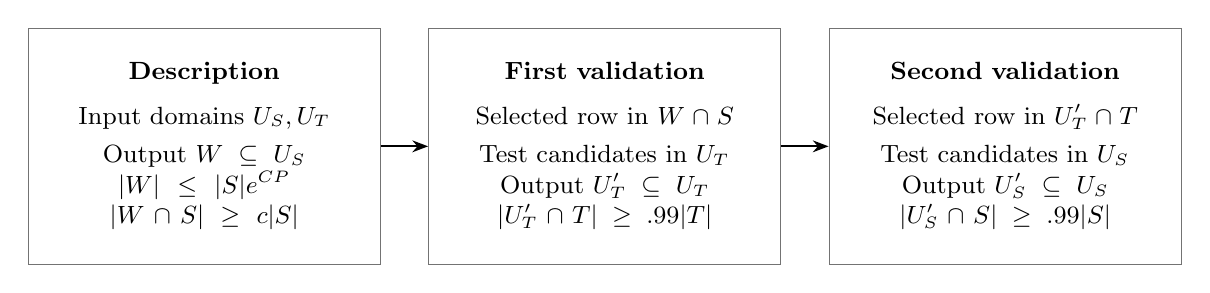
\begin{tikzpicture}[
  validationstage/.style={draw=black!55,align=center,text width=4.05cm,
    minimum height=3cm,inner sep=6pt,font=\small},
  flow/.style={-{Stealth[length=2mm]},thick},
  node distance=6mm]
\node[validationstage] (predict) {
  \textbf{Description}\\[5pt]
  Input domains $U_S,U_T$\\[3pt]
  Output $W\subseteq U_S$\\
  $|W|\le |S|e^{CP}$\\
  $|W\cap S|\ge c|S|$
};
\node[validationstage,right=of predict] (first) {
  \textbf{First validation}\\[5pt]
  Selected row in $W\cap S$\\[3pt]
  Test candidates in $U_T$\\
  Output $U_T'\subseteq U_T$\\
  $|U_T'\cap T|\ge .99|T|$
};
\node[validationstage,right=of first] (second) {
  \textbf{Second validation}\\[5pt]
  Selected row in $U_T'\cap T$\\[3pt]
  Test candidates in $U_S$\\
  Output $U_S'\subseteq U_S$\\
  $|U_S'\cap S|\ge .99|S|$
};
\draw[flow] (predict)--(first);
\draw[flow] (first)--(second);
\end{tikzpicture}
\caption{The description gives a first approximation; two separately
addressed validation tables give near-complete capture on both sides.
The second validation tests the original domain $U_S$, not $W$.
For either validation row, the constant-density comparison with iid
sampling holds at readiness and conditional on that row being produced,
not conditional on later success. No such comparison is asserted for
the description's accepted row.}
\label{geom:validation-figure}
\end{figure}


\begin{lemma}[The law of a produced test]\label{geom:produced-test}
Consider either test in Lemma~\ref{geom:validation}, conditional on
all data making that test ready, but not on any later event. Suppose its
hidden source $X_0$ is a subset of an original support $X$ with
$|X_0|\geq c|X|$. For every fixed opposite point $y$,
\begin{equation}\label{geom:exclusion-bound}
 \Prob\{\text{the test is produced and its ambient test excludes }y\}
 \leq Cq\frac{|X\cap N(y)|}{|X|}.
\end{equation}
Conditional on production, the row law is dominated by a constant times
the independent uniform row law on $X_0$. The bound
\eqref{geom:exclusion-bound} may be averaged over earlier readiness data
whenever its right-hand side is fixed.
\end{lemma}

\begin{proof}
Let $\nu$ be one proposal's law and $A$ its acceptance event. For
independent proposals and any deterministic cutoff $m$, the first
accepted row, conditional on there being one among the first $m$, has
law $\nu(\,\cdot\mid A)$. Indeed, the contribution of acceptance at
index $i$ is $(1-\nu(A))^{i-1}\nu(A)$ times that same conditional
law. Given that all entries lie in $X_0$, the proposal is an independent
uniform row on $X_0$, and the further acceptance probability is at least
$.9$. The claimed domination follows. Apply
\eqref{geom:pointwise-iid} and use
\[
 \frac{|X_0\cap N(y)|}{|X_0|}
 \leq c^{-1}\frac{|X\cap N(y)|}{|X|}.
\]
Multiplication by the probability of production can only decrease the
bound. No later success, including production of the other validation
test, has been conditioned on.
\end{proof}

\subsection{Reduction from higher projective dimensions}

\begin{proposition}[Repeated projection]\label{geom:projection}
For $j\geq4$, assume Lemma~\ref{geom:description} in projective
dimension $j-1$, for every fixed value of its hypothesis constant.
Then the lemma holds in dimension $j$.
\end{proposition}

\begin{proof}
For a point $z$ represented by a vector line $\langle z\rangle$, the
quotient vector space has dimension $j$ and hence projectivization
$\PG(j-1,q)$. Projection maps a point different from $z$ to its
image in this quotient; its fibers are the $q$ noncentral points of
lines through $z$. The dual operation retains hyperplanes containing
$z$, identified with hyperplanes of the quotient. Write $S_0,T_0$ for
the projected $S\setminus\{z\}$ and the cut $T\cap z^\perp$.
Apply the same operations to the decoder domains.

Lifting a quotient cap can enlarge it by a factor $q$, the size of a
projection fiber. We remove that enlargement by intersecting caps from
eight projections, always using the original $S,T$. At a given call let
$A\subseteq U_S$ be the intersection of all caps lifted so far, initially
$A=U_S$. The next center will preserve almost all of $S$ and limit
collisions among the points of this current set $A$; the latter property
makes successive intersections contract.
There exists a center, chosen before that
call's fresh tables, satisfying
\begin{equation}\label{geom:center-properties}
 \begin{aligned}
 |T_0|&\asymp |T|/q,&
 |U_T\cap z^\perp|&\leq C|U_T|/q,\\
 |S_0|&\geq(1-o(1))n,&
 e(S_0,T_0)&\leq C\tau |S_0||T_0|/q,\\
 \operatorname{coll}_z(A)&\leq C|A|^2/q^{j-1}.&&
 \end{aligned}
\end{equation}
Here $\operatorname{coll}_z(A)$ counts unordered distinct pairs of
$A\setminus\{z\}$ with the same projection.

To prove existence, choose $z$ uniformly in the ambient point space.
The variance identity gives
\[
 \Prob\left\{\left||T\cap z^\perp|-p_j|T|\right|
                >\frac{|T|}{3q}\right\}
 \leq Cq/|T|=o(1).
\]
Here $|T|\geq q^{(j+1)/2}e^{-b/2}\gg q$, and replacing the constant
$1/3$ by any other fixed positive constant is harmless. Markov's
inequality gives the stated cut-domain bound with arbitrarily high
fixed probability. A distinct pair projects together only if $z$ lies
on its joining line, an event of probability at most
$(q+1)/Q_j=O(q^{1-j})$. Thus
\[
 \E\operatorname{coll}_z(A)\leq C|A|^2/q^{j-1},\qquad
 \frac{\E\operatorname{coll}_z(S)}{n}
 \leq Cq^{(3-j)/2}=o(1).
\]
The latter implies projection loss $o(n)$ with probability $1-o(1)$:
each nonempty fiber loses at most its number of unordered pairs, and
omitting $z$ loses at most one more point. Finally, an original
incidence survives the dual cut with probability $p_j\leq C/q$.
Its expected count before collapsing fibers is at most
$C\tau n|T|/q^2$, and collapsing cannot increase it. A union bound,
using large fixed constants in the three Markov bounds, proves
\eqref{geom:center-properties}. This reasoning is valid for every
realized current $A$: fix that set and all earlier data, then combine
the two events of probability $1-o(1)$ with the three Markov bounds.
Their constants can be chosen so that the simultaneous event has
positive probability. Choose a center in that event before exposing
any of the fresh tables used by this call.

Transmit $z$ in $O(\sigma)$ bits and use a fixed coordinate convention
on the quotient. The new product is at least $q^je^{-b-O(1)}$ and the
density at most $C\tau/q$. The projected $S$ domain has size at most
$|U_S|$, whereas $|S_0|=(1-o(1))n$; on the other side both domain and
support shrink by comparable factors $q$. Hence both logarithmic gaps
increase by $O(1)$. These are the induction hypotheses, with changed
fixed constants. Reorient if necessary, apply induction, and then
Lemma~\ref{geom:validation}, which returns caps on both quotient
sides. In particular, the projected $S$ cap captures $.99|S_0|$ and
has size at most
\[
 \frac{Cq^j}{|T_0|}\leq \frac{Cq^{j+1}}{|T|}
 \leq m_0:=ne^{C_3P}.
\]
Lift this cap, excluding $z$, and intersect it with $A$.
The original support loss is at most $.01n$, plus the $o(n)$ total
fiber excess, plus one possible center: among the lost images there
are at most $.01|S_0|$ first preimages, and all additional preimages
are charged to $n-|S_0|-\boldsymbol 1_{\{z\in S\}}=o(n)$.
This bound concerns the original $S$, not merely the points retained
by earlier calls. Thus each call loses fewer than $.02n$ of its
original points, and losses from intersecting the lifted caps add.

The first call gives $|A_1|\leq qm_0$. For any later call let $k_i$
be the retained nonzero fiber sizes; there are at most $m_0$ of them.
Cauchy--Schwarz and \eqref{geom:center-properties} give
\[
 \begin{split}
 |A_{\mathrm{new}}|
 &\leq m_0+\sum_i(k_i-1)
 \leq m_0+\sqrt{m_0\sum_i k_i(k_i-1)}\\
 &\leq m_0+C|A|\sqrt{m_0/q^{j-1}}.
 \end{split}
\]
By \eqref{geom:product-upper}, the last coefficient is
\[
 \rho\leq e^{C_4P}q^{(3-j)/4}\leq q^{-1/4+o(1)}.
\]
After seven further calls,
$|A_8|\leq m_0(1+\rho+\cdots+\rho^6)+qm_0\rho^7=O(m_0)$,
while more than half of the original $S$ remains. Eight calls multiply
the cost and failure bounds by fixed constants. The center at each
stage depends only on data available before its fresh tables, so all
conditional failure bounds apply. The set $W=A_8$ proves the result.
\end{proof}

\subsection{Preparing dimensions two and three}

The remaining analysis will use a retained support $S'$ and, in one
case, an ordered list of planes. The list isolates planar concentrations;
for a query point we remove the training cell in its first containing
plane before measuring overlaps.

\begin{proposition}[Low-dimensional preparation]\label{geom:preparation}
Suppose \eqref{geom:sparse-hypotheses} holds with $j\in\{2,3\}$ and
$n=|S|\leq|T|$. Either enumeration already proves
Lemma~\ref{geom:description}, or the following preparation costs
$O(q+\sigma)$ bits. In dimension three there is also a possible
reduction to the dimension-two description lemma, with the same final
cost, size, capture, and failure bounds as
Lemma~\ref{geom:description}.

In the case not resolved by enumeration or that reduction, we have
$n>100qP$, a retained set $S'\subseteq S$ of size
$n'\in[n/2,n]$, and either an empty list or an ordered plane list
$\Pi_1,\ldots,\Pi_J$ in $\PG(3,q)$. In the latter case the sets
\begin{equation}\label{geom:cells}
 C_i=(S\cap\Pi_i)\setminus\bigcup_{h<i}\Pi_h
 \quad(1\leq i\leq J)
\end{equation}
partition $S'$, have nonincreasing sizes, and satisfy
$|C_i|<.04n'$. The decoder knows the list and all cell sizes, but need
not know $S'$ or the cells themselves.

Write
\begin{equation}\label{geom:lowdim-parameters}
 n=q^{1+v},\quad g=(v-1/2)\sigma,\quad
 \chi=P/100,\quad\chi_0=P/10000,\quad B=q^j/n'.
\end{equation}
For every ambient query point $x$, define $O_x$ to be the cell $C_i$
of its earliest containing listed plane, and $O_x=\varnothing$ if
there is none. Define
\begin{equation}\label{geom:outside-support}
 f_x=|O_x|/n'\leq .04,\qquad
 X_x=S'\setminus(O_x\cup\{x\}).
\end{equation}
If no list is present, $O_x=\varnothing$ for all $x$. When
$j=3$ and $g>\chi_0$, the preparation additionally ensures either
\begin{enumerate}[label=(\roman*)]
 \item every plane meets $S'$ in fewer than
 $K_p=n^{4/3}q^{-1}e^{-g/5}$ points and the list is empty; or
 \item the list is present and
 $J\leq n/K_p=q^{1/2}e^{-2g/15}$.
\end{enumerate}
\end{proposition}

\begin{proof}
If $n\leq100qP$, transmit $n$ and the index of $S$ among the
$n$-subsets of $U_S$. The cost is at most
\[
 O(\sigma)+\log_2\binom{|U_S|}{n}
 \leq C\bigl(\sigma+n(d_S+1)\bigr),
\]
which is within the description budget. It gives $W=S$ without
failure. Assume henceforth $n>100qP$, so $v>0$.

When $j=3$ and $g>\chi_0$, greedily choose a plane richest in the
remaining points of $S$, provided it contains at least $K_p$ of them,
and remove those points. Stop as soon as at least $n/2$ points have
been removed or no qualifying plane remains. In the first case retain
the captured prefix, with its list and cells; in the second retain the
residual without a list. Otherwise retain all of $S$ without a list.
The asserted size and cap properties follow directly from the stopping
rule. Greedy maximality makes the removed cell sizes nonincreasing.
Since each removal has size at least $K_p$, the list has length at
most $n/K_p=q^{1/2}e^{-2g/15}\leq q^{1/2}$. Plane identifiers and
cell sizes each cost $O(\sigma)$ bits, so the list costs $O(q)$.

Suppose now that a retained list has a cell of size at least $.04n'$,
and let $\Pi$ be its containing plane. Then
$S_1=S\cap\Pi$ has size at least $.02n$. The original sparsity and
Markov's inequality imply that at least half of $T$ consists of
hyperplanes having incidence proportion at most $C\tau/q$ into
$S_1$. For large $q$ this is less than one, so their restrictions to
$\Pi$ are nonzero projective covectors. Each nonzero projective
restriction has exactly $q$ projective lifts: normalize its restriction
to a fixed representative and choose the coefficient on a complement
of the vector space underlying $\Pi$.

Group the retained lifts by their restriction multiplicities. One
dyadic class $[h,2h)$, with $1\leq h\leq q$, carries at least
$c|T|/\sigma$ lifts. If $T_1$ is its set of distinct restrictions,
then
\[
 |T_1|\geq c|T|/(h\sigma),\qquad
 |S_1||T_1|\geq q^3e^{-b-O(\log\sigma)}.
\]
Every member of $T_1$ has incidence proportion at most $C\tau/q$
into $S_1$, since all its lifts have identical incidences there.
Transmit $\Pi$ and $h$. Use decoder domains $U_S\cap\Pi$ and the
nonzero restrictions having at least $h$ lifts in $U_T$. The latter
has size at most $|U_T|/h$, so its logarithmic gap increases by
$O(\log\sigma)$; the former gap increases by $O(1)$.

Apply the dimension-two description, with reorientation if needed,
and then Lemma~\ref{geom:validation}. The resulting cap on $S_1$
has size at most
\[
 \frac{Cq^3}{|T_1|}
 \leq\frac{Cq^4\sigma}{|T|}
 \leq Cn\sigma e^b\leq ne^{CP}
\]
and captures $.99|S_1|\geq cn$ points of $S$. Its cost is within
the required budget because $\log\sigma=o(P)$; its failure
probability has the required order. This deals with every large cell.
All other cases have the stated small-cell preparation. Notice that
$O_x$ is a subset of the training support: even when $x\notin S'$,
the earliest containing plane still specifies the same whole cell.
\end{proof}

\subsection{A polynomial bound for rich lines}

We give the needed algebraic estimate with its richness and
characteristic hypotheses explicit. It is used only when the line
richness substantially exceeds the cubic-root scale and planar
concentration cannot account for many rich lines. The interpolation
and tangent-plane method has antecedents in
\cite{GuthKatz2010,ElekesKaplanSharir2011}. Positive-characteristic
obstructions are discussed in \cite{EllenbergHablicsek2016}; here the
argument keeps every relevant surface degree below the characteristic.

\begin{lemma}[Rich lines with a plane cap]\label{geom:rich-lines}
Let $q$ run through sufficiently large primes. Let $\mathcal S$ be
at most $n\leq Cq^2$ points of $\PG(3,q)$, with at most $K_p$
points in every projective plane. Let $M>0$ satisfy
\begin{equation}\label{geom:rich-regime}
 \frac{M^3}{n}\longrightarrow\infty,\qquad
 \frac{M^2}{K_p}\longrightarrow\infty,\qquad
 cq\leq\frac nM\leq Cq^{41/40}.
\end{equation}
Then at most $Cn/M$ projective lines contain at least $M$ points of
$\mathcal S$. The constant is uniform once the displayed limits hold
uniformly in the family under consideration.
\end{lemma}

\begin{proof}
Work over the algebraic closure $\mathbb K$ of $\mathbb F_q$.
Choose an affine chart containing all points of $\mathcal S$, which
is possible because $\mathbb K$ is infinite. The plane cap remains
valid for planes over $\mathbb K$: rational points on such a plane
have rational vector-span dimension at most three. Otherwise four
linearly independent rational representatives would remain independent
over $\mathbb K$. The points therefore lie in an $\mathbb F_q$-plane
and obey the same cap.

Independently sample each point with probability
$A\sqrt{n/M^3}=o(1)$, where $A$ is a sufficiently large fixed
constant. The expected sample count on any $M$-rich line is at least
$A\sqrt{n/M}\geq cA\sqrt q$. There are at most $n^2$ lines to
test, since $M\to\infty$ and two distinct points determine a line.
Binomial tails and a union bound show that, simultaneously with
positive probability, every rich line contains more than
$(A/2)\sqrt{n/M}$ sampled points, and the total sample has size at
most $2A(n/M)^{3/2}$. The latter assertion follows from an upper
binomial tail, or from stochastic domination if $|\mathcal S|<n$.

There are $\binom{D+3}{3}$ monomials of degree at most $D$ in three
variables. Solving the homogeneous linear system requiring vanishing
at the sample therefore gives a nonzero polynomial of degree at most
$CA^{1/3}\sqrt{n/M}$. Choose $A$ large enough that this degree is
smaller than the guaranteed number of sampled points on each rich
line. Restriction to a line is a univariate polynomial, so it vanishes
identically there. Replace the polynomial by its squarefree part.
Its degree $D_0$ satisfies
\begin{equation}\label{geom:interpolating-degree}
 D_0=O(\sqrt{n/M})=o(M),\qquad
 D_0\leq Cq^{41/80}<q.
\end{equation}

We now count three groups of rich lines. Plane factors are controlled
by the plane cap. Among the other lines, those with few points incident
to three lines are controlled by the total point count. The remaining
lines will lie in the common zero set of the nonplane surface and an
auxiliary polynomial coprime to it, whose degrees bound their number.

First count rich lines lying in plane factors. There are at most
$\binom{D_0}{2}$ lines lying in two distinct such planes. For one
plane let $u$ be the number of remaining rich lines it contains.
Select $M'=\lfloor M\rfloor$ points of $\mathcal S$ on each.
If $r_a$ is the number of selected occurrences at point $a$, then
\[
 \sum_a r_a=uM',\qquad
 \sum_a r_a^2\leq uM'+u(u-1).
\]
The second inequality uses the fact that two distinct lines meet in
at most one point. Cauchy--Schwarz and the plane cap give
\[
 (uM')^2\leq K_p\bigl(uM'+u(u-1)\bigr).
\]
For $u>0$ this implies
$u\leq K_pM'/((M')^2-K_p)=o(M')$. Remove from each selected line
its intersections with all other plane factors, losing at most $D_0$
points. The remaining union in this plane has size at least
\[
 u(M'-D_0)-\binom u2\geq uM'/2.
\]
Such unions for different planes are disjoint. Thus the plane factors
account for $O(n/M+D_0^2)=O(n/M)$ rich lines.

Let $F_0$ be the squarefree product of the nonplane irreducible factors.
Every as yet uncounted rich line lies on $F_0$: the coordinate ring of
a line is an integral domain, so vanishing of a product on the line
implies vanishing of one factor. If there are no such factors we are
done. For coordinate vectors $e_1,e_2,e_3$, form
\begin{equation}\label{geom:flatness-polynomials}
 Q_{ij}=(e_i\times\nabla F_0)^{\mathsf T}
       \operatorname{Hess}(F_0)(e_j\times\nabla F_0),
 \qquad 1\leq i,j\leq3.
\end{equation}
At a point on at least three of the remaining lines, all $Q_{ij}$
vanish. At a singular point this follows from the gradient factors.
At a nonsingular point, the three distinct line directions lie in the
two-dimensional tangent vector space. Restricting $F_0$ to each line
shows that its Hessian quadratic form vanishes on each direction. A
binary quadratic vanishing on three distinct projective directions is
zero; since the characteristic is odd, its associated bilinear form
is also zero. The vectors $e_i\times\nabla F_0$ span that tangent
space, proving the assertion.

Among incidences with points of $\mathcal S$, points on at most two
remaining lines account for at most $2n$ incidences. Hence all but
$O(n/M)$ remaining rich lines have at least $M/2$ points incident
with three or more remaining lines. Since
$\deg Q_{ij}<3D_0=o(M)$, every such line lies on every $Q_{ij}$.

To obtain a polynomial coprime to $F_0$, we must show that the
$Q_{ij}$ do not all vanish identically on any of its irreducible
components. The reason is local: their vanishing makes all second
derivatives of a smooth formal graph zero, while the degree bound
below the prime characteristic forces a plane factor.

We claim that no irreducible factor $F$ of $F_0$ divides all these
polynomials. Its degree is less than the prime characteristic $q$,
so a nonconstant $F$ has a nonzero partial derivative. Rename its
variable $z$, and write the other variables as $x_1,x_2$. By
squarefreeness, $F$ and $(F_0)_z$ are coprime in
$\mathbb K(x_1,x_2)[z]$. Indeed, modulo $F$ the derivative is
$F_z(F_0/F)$, and neither factor is divisible by $F$. Clearing a
univariate Bezout identity gives
\[
 A F+B(F_0)_z=a(x_1,x_2)\ne0
\]
with polynomial coefficients. Choose $x_1,x_2$ so that $a$ and
the leading coefficient of $F$ in $z$ are nonzero. A root in $z$
then gives a point on $F$ where $(F_0)_z\ne0$.

Translate this point to the origin. The invertible coefficient of
$z$ in $F_0$ determines, recursively by total degree, a unique formal
series $z=h(x_1,x_2)$ with $F_0(x_1,x_2,h)=0$. The other factors
are units on this branch. If $F$ divided every $Q_{ij}$, those
polynomials would vanish after this substitution. To see the tangent
space statement over the formal series ring explicitly, write
$g=\nabla F_0(x_1,x_2,h)$. Its third coordinate $g_3$ is a unit,
and the kernel of the row vector $g$ has basis
\[
 t_1=(1,0,-g_1/g_3),\qquad t_2=(0,1,-g_2/g_3).
\]
Moreover $e_2\times g=g_3t_1$ and $e_1\times g=-g_3t_2$.
The vanishing $Q_{ij}$ therefore makes the Hessian bilinear form
zero on this entire formal tangent module. Twice differentiating
$F_0(x_1,x_2,h)=0$ gives
\[
 (F_0)_z h_{ab}=0\quad (a,b\in\{1,2\}),
\]
so all second partial derivatives of $h$ vanish. For a monomial
$x_1^u x_2^v$ of total degree less than $q$, these conditions require
\[
 u(u-1)=uv=v(v-1)=0\pmod q.
\]
Only the constant and linear monomials satisfy these conditions.
Writing $h_1$ for the affine-linear part, we obtain
$h-h_1\in(x_1,x_2)^q$. Thus the polynomial
$F_0(x_1,x_2,h_1)$ vanishes to order at least $q$. Its degree is
less than $q$, so it is identically zero. The plane $z=h_1$ would
be a factor of $F_0$, a contradiction. This proves the claim.

Because $\mathbb K$ is infinite, a constant linear combination $Q$
of the $Q_{ij}$ can be chosen coprime to $F_0$: for each of its
finitely many irreducible factors, combinations divisible by that
factor form a proper linear subspace of the coefficient space. We
finish by justifying the elementary common-line bound used here.

If coprime polynomials in three variables have degrees $D_1,D_2$,
they contain at most $2D_1D_2$ common lines. To see this, take any
finite collection of such lines and choose coordinates $(t,u,v)$
with $t$ nonconstant on each. Over the fraction fields in the other
two variables, univariate coprimality gives cleared identities
\[
 A F+B G=a(t,u)\ne0,\qquad
 C F+D G=b(t,v)\ne0.
\]
For a generic $c\in\mathbb K$, both right-hand sides remain
nonzero polynomials after $t=c$. Any common factor of the sliced
polynomials would divide both a polynomial in $u$ alone and one in
$v$ alone, and hence would be constant. Choose the slice also to
meet the selected lines in distinct points; only finitely many
values are forbidden by pairwise intersections of lines.
Choose coordinates on this slice so that these points have distinct
first coordinates. The resultant eliminating the second coordinate
is nonzero by coprimality and has degree at most $2D_1D_2$ in the
first coordinate. Indeed its Sylvester determinant has at most
$D_2$ columns with coefficients of degree at most $D_1$, and at
most $D_1$ columns with coefficients of degree at most $D_2$.
It vanishes at each of the distinct first coordinates, bounding
the collection. If both sliced polynomials omit the second
coordinate, their univariate coprimality gives no common point.
If just one omits it, say it is $f(u)$ and the other has degree
$m>0$ in the second coordinate, the resultant is $f(u)^m$;
it is again nonzero and vanishes at every common point.
As this bounds every finite collection, it bounds all common lines.

Apply the bound to $F_0,Q$, whose degrees are at most $D_0$ and
$3D_0$. The remaining lines number $O(D_0^2)=O(n/M)$. Together
with the earlier exceptional lines this proves the lemma.
\end{proof}

\subsection{Radial lines and overlap graphs}

The next two lemmas quantify the benefit of removing $O_x$. Planes
through a query point can overlap along a line, but after this removal
there are few lines carrying substantial retained mass, except at a
small set of query points.

\begin{lemma}[Radial rich lines]\label{geom:radial}
Consider the dimension-three output of
Proposition~\ref{geom:preparation}. A line $\ell$ through a query
point $x$ has strength
\[
 a_\ell(x)=q|X_x\cap\ell|/n'.
\]
Outside one exceptional set of $o(n)$ ambient points, simultaneously
for dyadic $a\in[q^{-10},2]$,
\begin{equation}\label{geom:radial-count}
 \#\{\ell\ni x:a_\ell(x)\geq a\}
 \leq q^{2-2v}e^\chi a^{-100}.
\end{equation}
In addition, whenever $g>\chi_0$ and $a>e^{-g/20}$ with
$0<a\leq2$, the total number of ambient center--line pairs
$(x,\ell)$ having strength at least $a$ is at most $Cq^2/a^2$.
\end{lemma}

\begin{proof}
The radial lines partition $X_x$, so their total strength is at most
$q$. Thus there are at most $q/a$ qualifying lines through any
center. Comparing this with \eqref{geom:radial-count} reduces to
\[
 e^{2g}a^{99}\leq e^\chi.
\]
This holds for $g\leq\chi_0$ and large $q$, since $a\leq2$ and
$2\chi_0<\chi$. It also holds when $g>\chi_0$ but
$a\leq e^{-g/20}$.

In the remaining regime put $M=n'a/q$. Since $n'\geq n/2$ and
$n=q^{3/2}e^g$,
\[
 \frac M{n^{1/3}}\geq c e^{(2/3-1/20)g},\qquad
 \frac{M^2}{K_p}\geq c e^{(2/3+1/10)g}.
\]
Also $cq\leq n/M\leq Cqe^{g/20}$, and
\eqref{geom:product-upper} gives $g\leq\sigma/2+O(1)$.
Hence all hypotheses of Lemma~\ref{geom:rich-lines} hold uniformly.
In the capped residual case, that lemma gives $Cn/M\leq Cq/a$
rich lines; each has $q+1$ rational centers. This yields at most
$Cq^2/a\leq Cq^2/a^2$ relevant pairs.

Suppose instead that the plane list is retained. Here own-cell removal
will force the center of a surviving rich line into a plane earlier
than the first listed plane containing that line. This gives a bound
on its possible centers. First, the list length satisfies
\[
 \frac JM\leq C e^{-(1+2/15-1/20)g}=o(1).
\]
A relevant line must be contained in a listed plane, since otherwise
it meets the union of the list in at most $J<M$ points. Let $i$
be its first containing plane. Earlier planes contribute at most
$J$ points to this line and later cells contribute none, so
$|C_i\cap\ell|\geq M-J\geq M/2$. Its center must be in an
earlier plane: otherwise $O_x=C_i$, leaving at most $J<M$ points
on this line in $X_x$. Since the line is not contained in any
earlier plane, there are at most $i-1$ possible centers for it.

Put $f_i=|C_i|/n'$. Fix a sufficiently large constant $C_0$.
If $a>C_0f_i$, the mean number of $C_i$ points on a line of
$\Pi_i$ is at most $2f_i n'/q$, much less than $M/2$.
The projective-plane incidence variance bounds the number of lines
with at least $M/2$ points by
\[
 \frac{Cq|C_i|}{M^2}
 \leq Cq^{2-v}f_i/a^2.
\]
Multiplying by at most $i$ centers and summing gives
\[
 Cq^{2-v}a^{-2}\sum_i i f_i
 \leq Cq^{2-v}J/a^2\leq Cq^2/a^2,
\]
because $\sum_i f_i=1$ and $J\leq q^v$. In the other case
$a\leq C_0f_i$, nonincreasing cell fractions and their unit sum
imply $i\leq C_0/a$; there are at most $C_0/a$ such indices.
Each corresponding plane has $O(q^2)$ lines and each line at
most $i$ possible centers. Their total is again $O(q^2/a^2)$.
This proves the center--line bound in all remaining cases.

For a fixed dyadic threshold, divide that bound by the right-hand
side of \eqref{geom:radial-count}. The number of centers where
the latter fails, divided by $n=q^{1+v}$, is at most
\[
 Cq^{v-1}e^{-\chi}a^{98}.
\]
Since $v\leq1+O(1/\sigma)$ and the sum of $a^{98}$ over all
dyadic $a\leq2$ is bounded, the union of these exceptional sets
has size $o(n)$, as asserted.
\end{proof}

\begin{lemma}[Overlap bounds for pencils]\label{geom:overlap}
Use the prepared data of Proposition~\ref{geom:preparation} in
dimension $j=2$ or $3$. For a query point $x$, let $\mathcal H_x$
be any family of hyperplanes through $x$ such that
\[
 \lambda'_H:=q|X_x\cap H|/n'\leq2\quad(H\in\mathcal H_x).
\]
For distinct $H,H'\in\mathcal H_x$ put
$\theta_{HH'}=q|X_x\cap H\cap H'|/n'$.
Let $E_a$ be the number of ordered pairs with $\theta_{HH'}\geq a$
and let $\Delta_a$ be the maximum degree of this graph. Outside
$o(n)$ ambient centers, simultaneously for dyadic
$a\in[q^{-10},2]$ and for every such family,
\begin{equation}\label{geom:overlap-bounds}
 E_a\leq B^2e^{2\chi}a^{-200},\qquad
 \Delta_a\leq Be^{2\chi}a^{-200}.
\end{equation}
Let $p$ be any even integer in
$[10000\sigma/P,10000\sigma/P+2]$ and put
$t_*=1/(100p)$. Outside a further set of at most $ne^{CP}$ ambient
centers, also
\begin{equation}\label{geom:strong-degree}
 \Delta_{t_*}\leq Be^{-3P}.
\end{equation}
The further exceptional set is used only for ambient output-size
control, not for support capture.
\end{lemma}

\begin{proof}
In dimension two, two distinct hyperplanes in the pencil are lines
intersecting only at $x$. Because $x\notin X_x$, all overlaps are
zero and all claims follow. Consider dimension three. The
intersection of two distinct planes through $x$ is a radial line;
each radial line belongs to $q+1$ planes and therefore accounts for
at most $Cq^2$ ordered pairs. Lemma~\ref{geom:radial} gives
\[
 E_a\leq Cq^{4-2v}e^\chi a^{-100}
 \leq B^2e^{2\chi}a^{-200}.
\]
The last inequality uses $B=q^3/n'\asymp q^{2-v}$ and $a\leq2$;
the factor $e^\chi$ absorbs fixed constants. Within one plane,
the radial lines partition its points other than $x$, so the sum
of their strengths is at most $2$. There are at most $2/a$
qualifying lines, each giving at most $q$ other planes. Thus
\begin{equation}\label{geom:crude-degree}
 \Delta_a\leq Cq/a.
\end{equation}
Since $B\geq cq$, this implies the second bound in
\eqref{geom:overlap-bounds}.

For the stronger assertion, $\log(1/t_*)=O(\log\sigma)=o(P)$.
If $(v-1)\sigma<-4P$, then
\[
 Be^{-3P}\geq cq e^P\geq Cq/t_*
\]
for large $q$, so \eqref{geom:crude-degree} suffices at every
center. Otherwise $n\geq q^2e^{-4P}$ and
$g\geq\sigma/2-4P>\chi_0$. Moreover
$t_*\gg e^{-g/20}$. The center--line estimate of
Lemma~\ref{geom:radial}, which does not require a dyadic threshold,
bounds the number of centers lying on even one radial line of
strength at least $t_*$ by
\[
 Cq^2/t_*^2\leq ne^{CP}.
\]
Remove these centers. At every remaining center
$\Delta_{t_*}=0$, proving \eqref{geom:strong-degree}.
\end{proof}

The geometry is now ready for the learning step. Its training support
is $S'$, the ordered plane data are known to the decoder, and the
own-cell rule in \eqref{geom:outside-support} is available for every
query point. Removing up to half of $S$ changes the sparse-incidence
bound by at most a factor of two. The overlap estimates are uniform
over all allowed pencil subfamilies, so those families may be selected
later using the prepared supports. Proposition~\ref{learn:short-row}
uses precisely these inputs to produce the cap required by
Lemma~\ref{geom:description}; the stronger ambient exceptional set
is never charged against support capture.

\section{Learning a sparse support from a short row}
\label{learn:section}

The remaining low-dimensional description problem is the following.
A set $S$ has unusually few incidences with a large opposite set $T$.
We want a short message describing a set that captures a fixed fraction
of $S$ and is not much larger than $S$. The decoder does not know either
support. We first construct the desired set from a random row of points
of a prepared subset of $S$, and then implement that row by searching a
public table of proposals from the known domain.

Two estimates have different roles. A second moment will show that the
test retains most points of the hidden support. A higher moment will
exclude almost all unwanted ambient points. Keeping these roles separate
is essential: some geometric exceptions allowed in the ambient estimate
are too large to discard from the support itself.

\subsection{The prepared input and the sampling test}

Use the parameters of Equation~\eqref{base:parameters}, with
$\sigma=\log q$, and put
\begin{equation}\label{learn:auxiliary-parameters}
 \chi=P/100,\qquad \xi=L/100,\qquad
 p\in[10000\sigma/P,10000\sigma/P+2]\cap2\mathbb Z,
 \qquad t_*=(100p)^{-1}.
\end{equation}
Here $p$ is a moment order, not the characteristic; the field is $\F_q$
with $q$ prime. In particular,
\begin{equation}\label{learn:scale-use}
 b+P\tau=o(L),\quad R\log L=o(P),\quad
 \log\sigma=o(L),\quad R\gg\log(p+2),\quad P=o(\sigma).
\end{equation}
These relations follow from Lemma~\ref{base:scale-comparisons} whenever
$b=O(K_*)$ and $\tau=O(\sigma^{-100\beta})$.

We specify the geometric input to this section. Let $j\in\{2,3\}$,
let $S,T$ be nonempty sets in opposite projective spaces of dimension
$j$, and suppose that
\begin{equation}\label{learn:support-hypotheses}
 S\subseteq U_S,\qquad n=|S|\le |T|,\qquad
 |S||T|\ge q^{j+1}e^{-b},\qquad
 e(S,T)\le \frac{\tau}{q}|S||T|.
\end{equation}
The set $U_S$ is known to the decoder. Write
$d_S=\log(|U_S|/n)$. We only need to treat
$n>100qP$, since smaller supports can be enumerated.

The prepared support is a subset $S'\subseteq S$ of size
$n'\in[n/2,n]$. In dimension three there may also be an ordered list
of projective planes $\Pi_1,\ldots,\Pi_J$. Its cells are
\[
 C_i=S'\cap\bigl(\Pi_i\setminus\textstyle\bigcup_{a<i}\Pi_a\bigr).
\]
The list is allowed to be empty; in dimension two it is always empty.
The list and the sizes of its cells admit an $O(q)$-bit description, and
every cell has size at most $.04n'$. For an ambient point $x$, let
$O_x=C_i$ if $\Pi_i$ is the first listed plane containing $x$, and let
$O_x=\varnothing$ if there is no such plane. Set
\begin{equation}\label{learn:radial-definitions}
 f_x=|O_x|/n',\quad X_x=S'\setminus(O_x\cup\{x\}),\quad
 B=q^j/n',\quad n=q^{1+v}.
\end{equation}
Thus $0\le f_x\le .04$. Every line through $x$ is called a radial
line at $x$, and has strength
$a_\ell=q|\ell\cap X_x|/n'$.

For each $x$, consider any family of hyperplanes $H$ through $x$ with
$q|H\cap X_x|/n'\le2$. For two distinct members put
$\theta_{HH'}=q|H\cap H'\cap X_x|/n'$. Let $E_a$ be the number of
ordered distinct pairs with $\theta_{HH'}\ge a$, and let $\Delta_a$
be the largest number of such neighbors of one member. The geometric
preparation supplies a deterministic exceptional set $D_0$ of size
$o(n)$ such that, outside $D_0$, simultaneously for dyadic
$a\in[q^{-10},2]$,
\begin{equation}\label{learn:overlap-input}
 E_a\le B^2e^{2\chi}a^{-200},\qquad
 \Delta_a\le Be^{2\chi}a^{-200}.
\end{equation}
There is a further deterministic set $D_1$, of size at most
$n e^{C_0P}$, outside which, also excluding $D_0$,
\begin{equation}\label{learn:strong-degree-input}
 \Delta_{t_*}\le Be^{-3P}.
\end{equation}
The bounds apply to all the indicated families. In dimension two the
overlaps vanish, so both assertions hold without geometric exceptions.
Proposition~\ref{geom:preparation} establishes this prepared input after its
enumeration and large-cell reductions, with the overlap bounds supplied
by Lemma~\ref{geom:overlap}.

\begin{proposition}[Short-row description]\label{learn:short-row}
Fix the constants in \eqref{learn:support-hypotheses}, the bound on
$b/K_*$, the bound on $\tau\sigma^{100\beta}$, and $C_0$.
For every sufficiently large prime $q$, the prepared input just
specified has the following description scheme. Using a fresh public
table, it either declares failure or describes a set $W\subseteq U_S$
satisfying
\[
 |W|\le n e^{CP},\qquad |W\cap S|\ge c n.
\]
Failure has probability at most $C e^{-cq}$, and the message has at most
$CqP(d_S+1)+Cq+C\sigma$ bits. In particular this is within
$CqP(d_S+d_T+P)$ for any $d_T\ge0$.
The bounds are uniform in all supports and prepared inputs satisfying
the hypotheses, including inputs fixed by earlier random history before
the fresh table is sampled. The decoder uses only $U_S$, public
parameters, and the new message; it need not know $S$, $T$, or $S'$.
\end{proposition}

Mixing in Lemma~\ref{base:incidence} and the smaller-side orientation
give $n\le Cq^{(j+1)/2}$. Consequently the quantities used below obey
\begin{equation}\label{learn:elementary-sizes}
 \frac q{n'}<\frac1{50P},\qquad
 Q_{j-1}=O(B^2),\qquad B^{-1}\le e^{-P},\qquad
 v\le1+O(1/\sigma).
\end{equation}
The last bound will only be needed in dimension three.

We first sample from the hidden set $S'$. Take $R$ independent batches.
Each batch has Poisson size of mean $qL$, and, conditional on its size,
has independent uniform entries in $S'$. Equivalently, the numbers of
occurrences of the different point-batch pairs are independent Poisson
variables of mean $qL/n'$. Indeed the joint probability of prescribed
counts is obtained by multiplying the Poisson probability of their sum
by the multinomial probability conditional on that sum; the factorials
then factor over points. The total number of samples has mean $qP$.

For a hyperplane $H$ and a cell $C$, define
\[
 \lambda_H=\frac{q|S'\cap H|}{n'},\qquad
 \lambda_{H,C}=\frac{q|C\cap H|}{n'},\qquad f_C=\frac{|C|}{n'}.
\]
Call $H$ exceptional if $|\lambda_H-1|>.1$ or
$|\lambda_{H,C}-f_C|>.02$ for at least one cell; let $\mathcal E$
be this set. All other hyperplanes are typical. Let
\begin{equation}\label{learn:empty-set}
 Z=\{H\in\mathcal E:H\text{ has no sample in any batch}\},\qquad
 z=|Z|,\qquad z_x=|\{H\in Z:x\in H\}|.
\end{equation}
These objects are used by the encoder; the decoder will receive only
the integer $z$, not the hidden set $Z$.

For a query point $x$, put $b_x=e^{-L(1-f_x)}$, and let $N_r(A)$
denote the number of samples of batch $r$ in a point set $A$.
For each hyperplane through $x$, we multiply $R$ batch tests.
In each batch we center the emptiness indicator outside $O_x$ at $b_x$,
and set the test to zero if $O_x\cap H$ contains a sample. Thus a
hyperplane empty in every batch contributes $(1-b_x)^R$, whereas
any other hyperplane has product of absolute value at most $b_x$.
For typical hyperplanes, their normalized mass outside $O_x$ is close
to $1-f_x$.
Batch independence turns bounds on one-batch means and pair moments
into $R$th-power bounds. The overlap estimates then control the sum
over typical hyperplanes.
Define the score by
\begin{equation}\label{learn:score}
 A_x=\sum_{H\ni x}\prod_{r=1}^R
 \left[
 1_{\{N_r(O_x\cap H)=0\}}
 \left(1_{\{N_r((S'\setminus O_x)\cap H)=0\}}-b_x\right)
 \right].
\end{equation}
The random test includes every sampled point and every other point
with $A_x<z/(2q)$. Both factors inside the brackets belong to batch
$r$. Although the formula mentions hidden subsets, the decoder can
evaluate it from the samples, the plane list, the cell sizes, and $z$:
earliest membership in the list identifies each sample's cell and the
cell $O_x$, if present. The size $n'$ is transmitted as well.
The separate own-cell indicator also preserves the geometric benefit
of removing $O_x$: once its sample counts and the absence of a sample
at $x$ are fixed, the remaining randomness consists of independent
counts on the radial lines in $X_x$. We use this conditioning when
estimating the typical contribution.

\subsection{Regular pencils and empty exceptional hyperplanes}

The pencil at $x$ is the set of hyperplanes through $x$. We next discard
a small deterministic set of pencils on which squared deviations are
unusually concentrated. This is separate from all sampling events.

\begin{lemma}[Regular pencils]\label{learn:regular-pencils}
There is a deterministic set $D_2$ of size $o(n)$ such that, for
$x\notin D_2$, its pencil contains at most $Be^\xi$ exceptional
hyperplanes and satisfies
\[
 \sum_{H\ni x}\min\{1,(\lambda_H-1)^2\}\le Be^\xi,
 \qquad
 \sum_{H\ni x}\min\{1,(\lambda_{H,C}-f_C)^2\}\le Be^\xi
\]
for every cell $C$. The constants and the $o(n)$ estimate are uniform
over the prepared inputs. We call these pencils regular.
Moreover, for every regular pencil and its typical members, with
\begin{equation}\label{learn:outside-mass}
 \lambda'_H=\frac{q|H\cap X_x|}{n'},\qquad
 \delta'_H=\lambda'_H-(1-f_x),
\end{equation}
we have
\begin{equation}\label{learn:typical-bounds}
 .75\le\lambda'_H<2,\qquad |\delta'_H|\le .18,\qquad
 \sum_{\substack{H\ni x\\H\text{ typical}}}(\delta'_H)^2
 \le CBe^\xi.
\end{equation}
\end{lemma}

\begin{proof}
Weighted incidence variance gives
\begin{equation}\label{learn:total-variance}
 \sum_H(\lambda_H-1)^2\le CqB,\qquad
 \sum_H(\lambda_{H,C}-f_C)^2\le CqBf_C.
\end{equation}
The exact means differ from $1$ and $f_C$ by the factors
$qp_j=1-1/Q_j$, whose squared contributions satisfy the same bounds.
Summing over cells and using $\sum_C f_C\le1$ proves
\begin{equation}\label{learn:exceptional-size}
 |\mathcal E|\le CqB,\qquad
 \sum_{H\in\mathcal E}\lambda_H\le CqB.
\end{equation}
For the second assertion use Cauchy--Schwarz on
$\sum_{H\in\mathcal E}(\lambda_H-1)$.

For the clipped squared-deviation weight of a cell, the total weight is
at most $CqBf_C$ and each weight is at most one. Its pencil sums have
mean $O(Bf_C)$ and total squared deviation at most $Cq^jBf_C$, by
Lemma~\ref{base:incidence}. For sufficiently large $q$, exceeding
$Be^\xi$ therefore excludes at most
\[
 C\frac{q^jBf_C}{B^2e^{2\xi}}=Cn'f_Ce^{-2\xi}
\]
centers. Sum this estimate over cells, rather than multiplying by their
number. The full-deviation weight and the exceptional-indicator weight
have the same proof with fraction one. Their union is $D_2$.

For a typical hyperplane, removing $O_x$ subtracts a quantity within
$.02$ of $f_x$, when a cell is present. Removing $x$ subtracts at most
$q/n'$. Thus $\lambda'_H\ge .9-.04-.02-q/n'>.75$ and
$|\delta'_H|\le .1+.02+q/n'<.18$. The upper bound by 2 follows as well.
On typical hyperplanes the relevant squared deviations are already
below one. The inequality $(u+v+w)^2\le3(u^2+v^2+w^2)$ and regularity
give the last bound in \eqref{learn:typical-bounds}; the removed center
adds at most
$O(q^{j-1}(q/n')^2)=O(B)$ by \eqref{learn:elementary-sizes}.
\end{proof}

\begin{lemma}[The empty exceptional set]\label{learn:empty-exceptional}
There is a fixed $c_0>0$ such that, with probability at least
$c e^{-8P\tau}$,
\begin{equation}\label{learn:empty-good-event}
 z\ge z_{\min}:=c_0qB e^{-b-8P\tau},\qquad
 \sum_{H\in Z}\lambda_H\le .001z.
\end{equation}
For every $Z$ satisfying these two inequalities, at least $.99n'$
points of $S'$ have $z_x\le .1z/q$, whereas all but
$O(q^{j+1}/z)$ ambient points have $z_x\ge .8z/q$.
At a regular pencil, the exceptional-hyperplane part of
\eqref{learn:score} differs from $(1-b_x)^Rz_x$ by at most
$b_xBe^\xi=o(z_{\min}/q)$, uniformly in the samples, and
$(1-b_x)^R=1-o(1)$.
\end{lemma}

\begin{proof}
The average of $\lambda_H$ over $T$ is at most $2\tau$.
At least half of $T$ consequently has $\lambda_H\le8\tau$.
These hyperplanes are exceptional, and their number $m$ is at least
$c qB e^{-b}$ by \eqref{learn:support-hypotheses} and $n'\ge n/2$.
Each is empty with probability at least $a=e^{-8P\tau}$.
If $Y$ counts the empty members of this particular set, then
$0\le Y\le m$ and $\E Y\ge ma$. Therefore
$\Prob(Y\ge ma/2)\ge a/2$, without any independence assumption among
the hyperplanes. Choose $c_0$ small enough to obtain the first inequality
of \eqref{learn:empty-good-event} on this event.

By \eqref{learn:exceptional-size}, the expected contribution from
$\lambda_H\ge10^{-4}$ to $\sum_{H\in Z}\lambda_H$ is at most
$CqB e^{-10^{-4}P}$. Markov's inequality at $.0009z_{\min}$ bounds
the probability of a larger contribution by
\[
 C\exp\{b+8P\tau-10^{-4}P\}=o(e^{-8P\tau}).
\]
The remaining contribution is at most $.0001z$. Subtracting this
failure probability proves the asserted simultaneous event.

For fixed $Z$, incidence variance has mean $p_jz=(1-o(1))z/q$ and
total squared deviation at most $q^{j-1}z$. This gives the ambient
exception bound. On the hidden support, exact double counting gives
\[
 \sum_{x\in S'}z_x=\frac{n'}q\sum_{H\in Z}\lambda_H
 \le .001n'z/q,
\]
which proves the $.99n'$ assertion by Markov's inequality.

An exceptional hyperplane in $Z$ contributes $(1-b_x)^R$ to the score.
For any other exceptional member of the pencil, an own-cell hit makes
its product zero; otherwise an outside hit gives a factor $-b_x$,
and all other factors have absolute value at most one. Its contribution
has absolute value at most $b_x$. Regularity proves the error bound.
Finally $b_x\le e^{-.96L}$, so
$b_xBe^\xi\le Be^{-.95L}=o(z_{\min}/q)$ and $Rb_x=o(1)$ by
\eqref{learn:scale-use}.
\end{proof}

The empty hyperplanes thus give a score that is small on most of $S'$
and large on most ambient points. It remains to show that the typical
hyperplanes do not obscure this distinction. Write $T_x^*$ for their
contribution to \eqref{learn:score}.

\subsection{Conditional moments of the typical contribution}

Fix $x$ and condition on its being unsampled and on all point-batch
counts in $O_x\setminus\{x\}$. Denote these conditioning data by
$\mathcal O_x$; when $x\notin S'$, the unsampled condition is automatic.
Every assertion below is uniform over conditioning values of positive
probability. The own-cell multipliers in \eqref{learn:score} are now
fixed zeros or ones. Counts on $X_x$ are unchanged independent Poisson
variables. Grouping them by radial lines gives independent
line-batch schedules, with hit probability at most $La_\ell$ for
line $\ell$ in one batch. Distinct lines are disjoint in $X_x$ because
the center has been removed.

Temporarily omit a fixed own-cell multiplier and let
$X_H=1_{\{H\cap X_x\text{ empty in the batch}\}}-b_x$.
Its mean $u_H$ and its pair moments obey
\begin{align}
 u_H&=e^{-L\lambda'_H}-b_x,
 &|u_H|&\le Le^{-.75L}|\delta'_H|,\label{learn:one-mean}\\
 \E(X_HX_{H'})
 &=u_Hu_{H'}+e^{-L(\lambda'_H+\lambda'_{H'})}
                      (e^{L\theta_{HH'}}-1),\label{learn:one-covariance}\\
 |\E(X_HX_{H'})|
 &\le L^2e^{-.75L}(|\delta'_H\delta'_{H'}|+\theta_{HH'}),
 &\E X_H^2&\le2e^{-.75L}.\label{learn:one-bounds}
\end{align}
The covariance identity is the Poisson emptiness formula for a union.
For its bound, use
$\lambda'_H+\lambda'_{H'}-\theta_{HH'}\ge .75$ and
$e^u-1\le ue^u$ for $u\ge0$.

\begin{lemma}[Second moment]\label{learn:second-moment}
If $x\notin D_0\cup D_2$, then, conditional on $\mathcal O_x$,
\[
 \E\bigl((T_x^*)^2\mid\mathcal O_x\bigr)
 \le B^2e^{-.6P}.
\]
This assertion does not exclude the set $D_1$.
\end{lemma}

\begin{proof}
Batch independence raises the bounds in \eqref{learn:one-bounds} to
the $R$th power. Fixed zero-one multipliers cannot increase their absolute
values. By \eqref{learn:typical-bounds},
\[
 \sum_H|\delta'_H|^R\le CBe^\xi.
\]
For the overlap terms, \eqref{learn:overlap-input} and dyadic summation
give, for $R>200$,
\[
 \sum_{H\ne H'}\theta_{HH'}^R
 \le B^2\exp\{2\chi+O(R+\log\sigma)\}.
\]
Every positive overlap is at least $q/n'$ and at most 2, so it falls
within the available dyadic range. There are $O(\sigma)$ dyads. The
inequality $(u+v)^R\le2^{R-1}(u^R+v^R)$ handles their sum with the
deviation terms. The diagonal contributes at most
$Q_{j-1}(2e^{-.75L})^R$. Now use $Q_{j-1}=O(B^2)$,
$2\chi=.02P$, and $R\log L=o(P)$ to obtain the claimed exponent.
\end{proof}

\begin{lemma}[High moment]\label{learn:high-moment}
If $x\notin D_0\cup D_1\cup D_2$, then, conditional on
$\mathcal O_x$,
\[
 \E\bigl((T_x^*)^p\mid\mathcal O_x\bigr)
 \le B^p e^{-.1pP}.
\]
\end{lemma}

\begin{proof}
We expand into ordered $p$-tuples of typical hyperplanes and bound the
absolute expectation of every summand. The evenness of $p$ will permit
the final tail estimate. A tuple may contain repeated hyperplanes.
Among its distinct hyperplanes, join $H,H'$ when
$\theta_{HH'}>t_*$, and take the connected components of this graph.
A component consisting of one hyperplane appearing once in the tuple
is a \emph{simple singleton}. All other components are nonsimple.

\paragraph{Component expectations.}
A positive-strength radial line is external to the tuple if it is
contained in hyperplanes in different components. The sum of the
strengths of the external lines in any fixed tuple hyperplane is at
most $pt_*=.01$: assign each such line to one other tuple hyperplane
containing it, whose overlap is at most $t_*$. Condition further on
all external line-batch schedules. The remaining schedules affecting
different components are independent, and each hyperplane has internal
mass at least $.75-.01=.74$. Call a hyperplane touched in a batch if
one of its external lines has a hit in that batch.

For a nonsimple component, all factor magnitudes are at most one.
Keeping just the factors of one of its hyperplanes bounds its absolute
product expectation. In an untouched batch the expected absolute
factor is at most $2e^{-.74L}$; in a touched batch it is at most
$b_x\le e^{-.96L}$. Independence between batches consequently bounds
the entire component by
\begin{equation}\label{learn:nonsimple-attenuation}
 (2e^{-.74L})^R\le e^{-.7P}.
\end{equation}

For a simple singleton keep its signed expectation. Let
$\theta_{\max}$ be the largest overlap $\theta_{HH'}$ over the other
distinct hyperplanes $H'$ of the current tuple, taking zero if there
are none. It is not a maximum over the whole pencil. In an untouched
batch the mean has absolute value at
most
\[
 Le^{-.74L}(|\delta'_H|+p\theta_{\max});
\]
in every batch it has absolute value at most $2e^{-.74L}$.
Let $\mathcal B_H$ be the event that $H$ is touched in at least
$R/2$ batches. If it is not, at least $R/2$ factors have the sharper
bound. Since $p\theta_{\max}\le .01$, $R/2\ge200$, and
$R\log(2L)=o(P)$, the resulting bound for a simple singleton is
\begin{equation}\label{learn:simple-attenuation}
 e^{-.68P}\left(
 |\delta'_H|^{R/2}+(p\theta_{\max})^{200}+1_{\mathcal B_H}
 \right).
\end{equation}
The fixed own multipliers do not change either estimate.

We now sum these fixed-tuple bounds over the possible hyperplanes.
For each valid tuple, retain $e^{-.7P}$ per nonsimple component and
$e^{-.68P}$ per simple position, and expand the three terms in
\eqref{learn:simple-attenuation} at each simple position. The resulting
bounds are nonnegative. After averaging the external schedules, the
only remaining probabilistic factor in each term is the conditional
probability of the selected events $\mathcal B_H$ occurring together.
We will bound the sum of these terms after dividing by $B^p$.

The geometric choices have three forms. Nonsimple components are
counted either from a strong pair and a spanning tree or from repetitions
of one hyperplane; deviation and overlap terms use the corresponding
pencil bounds; the remaining hit events
are covered by static certificates. Each such certificate charges
any independent direction-batch hit event at most once. We construct
these certificates below and then verify the probability union bound.
These descriptions count moment terms and are not part of the
public-table message.

The combinatorial descriptions use only $p^{O(p)}$ choices of names,
partitions, and orders. Record the partition
of positions into equal hyperplane names, the partition of distinct
names into their strong components, and spanning trees and traversal
orders inside those components. Do not record the full strong graph.
For any geometric assignment its true graph determines whether these
recorded components are valid; an invalid assignment initially contributes
zero. Dropping such validity restrictions later only enlarges a positive
sum after the attenuation bounds have been assigned.

\paragraph{Nonsimple and deviation choices.}
For a component with at least two distinct hyperplanes, start with a
strong pair. By \eqref{learn:overlap-input}, its normalized count is
at most
\[
 e^{2\chi}(C/t_*)^{200}.
\]
Each later distinct vertex along its tree costs at most $e^{-3P}$ by
\eqref{learn:strong-degree-input}; a repeated position costs $1/B$.
For a component consisting of one hyperplane repeated, its first two
positions cost $Q_{j-1}/B^2=O(1)$, and further positions again cost
$1/B$. These counts are combined with
\eqref{learn:nonsimple-attenuation} once per component.

A deviation choice has weighted normalized sum at most
$Ce^\xi$ by \eqref{learn:typical-bounds}. Encode these and all nonsimple
components first. The remaining choices are overlap shifts and events
$\mathcal B_H$; their attenuation $e^{-.68P}$ has already been retained.

\paragraph{Overlap shifts.}
For an unencoded shift vertex, choose the name of a neighbor attaining
its largest positive overlap and a dyad $a\le\theta<2a$. Zero weights
need not be encoded. If the neighbor is encoded, the weighted normalized
count is at most
\[
 (2pa)^{200}\Delta_a/B.
\]
If it is not, encode the ordered pair with count
$(2pa)^{200}E_a/B^2$, dropping the neighbor's extra shift weight or
event requirement, each bounded by one. Both vertices retain their
attenuation. Equation~\eqref{learn:overlap-input} cancels $a^{200}$
in either case and gives at most $e^{2\chi}$ times polynomial overhead.
Summing dyads has the same type of overhead. Continue until all
unencoded vertices carry the event requirement $\mathcal B_H$.

\paragraph{Hit certificates and their probability weights.}
Fix a tuple and external schedules for which these remaining requirements
hold. We describe certificates witnessing enough of the hits to count
the tuple. Maintain two objects: a dictionary of radial directions whose
geometry is already recorded, and a set of charged direction-batch
events. On first introduction of a direction, charge one positive hit
event, except in the pair operation below, which charges 200 distinct
batches at once. Once that direction enters the dictionary, any later
reference to it imposes \emph{no new hit requirement}. In particular,
no direction-batch event is charged twice.

For a fixed tuple all charged events are external events, independent
under the conditional law given $\mathcal O_x$. Thus their joint
probability is at most the product of their $La_\ell$ weights. Keeping
$\min(1,La_\ell)$ would also be valid, but is unnecessary. From an
encoded hyperplane $H_0$, the weighted sum of choices of a new line
and a witnessing batch is at most
\begin{equation}\label{learn:line-charge}
 \sum_{r=1}^R\sum_{\ell\subset H_0}La_\ell
 =P\lambda'_{H_0}<2P.
\end{equation}
An old direction is specified by its dictionary index and requires no
new probability factor. If the current dictionary has $m$ directions,
these references have at most $m$ choices, each of incremental weight
one. A direction choice, allowing either a new charge or an old
reference, therefore has total weight at most $2P+m$. The construction
below keeps $m=O(p)$, so these extra choices enter only the polynomial
overhead.

\paragraph{Anchors and pairs.}
If an unencoded vertex has a touched direction shared with an encoded
hyperplane, encode it using that direction as an anchor. A new direction
is paid for by \eqref{learn:line-charge}; an old one is referenced.
Given the direction, there are at most $Cq^{j-2}$ hyperplanes through
it. The normalized geometric cost is therefore
\[
 O(q^{j-2}/B)=O(q^{v-1})=O(1).
\]
This uses $n'\asymp n$ and \eqref{learn:elementary-sizes}.
In dimension two there are no positive external directions, and no
such event requirements occur.

If no anchor is available but two unencoded vertices share external
hits in at least 200 distinct batches on directions in no encoded
hyperplane, encode this pair. Choose an overlap dyad, 200 witnessing
batches and one shared hit direction in each. These events are new and
distinct, outside the direction dictionary. For a fixed pair their
total probability weights, summed over the witness choices, are at
most $(2Pa)^{200}$. The normalized pair count in
\eqref{learn:overlap-input} then gives a cost at most
$e^{2\chi}(2P)^{200}$. Add the vertices and witness directions to the
encoded data. In dimension three the intersection direction of a
pair is unique; repeated use of that direction in distinct batches
still charges distinct independent events. Repeat the anchor and pair
operations whenever either applies.

\paragraph{The residual root set.}
Suppose $h$ vertices remain. Each has at least $R/2$ touched batches,
whose witnessing external directions are shared with residual vertices
only; otherwise an anchor would be available. Select one witness per
such batch. A fixed neighbor appears fewer than 200 times, and a fixed
direction appears fewer than 200 times. Either violation would permit
the pair operation. Greedily keeping one witness and discarding others
with its neighbor or its direction removes fewer than 400 witnesses.
Thus each residual vertex has at least $\lfloor R/800\rfloor$ witnesses
with distinct neighbors and distinct directions.

There exists a set of at most $h/10$ roots such that every nonroot has
two of these witnesses to roots. To prove this, select each vertex
independently with probability $1/20$. For any one witness list, the
probability of fewer than two selected neighbors is at most
$CR e^{-cR}$. Union over at most $p$ lists is $o(1)$ because
$R\gg\log(p+2)$. Markov's inequality bounds the probability of more
than $h/10$ selected vertices by $1/2$. The two conditions therefore
hold simultaneously with positive probability. If a residual set is
too small to have the displayed number of distinct neighbors, it could
not have reached this case in the first place.

Record the root names and choose their hyperplanes freely, dropping
their extra event requirements. A root has normalized cost
$Q_2/B=O(q^v)$. Encode each nonroot by two distinct directions in
its two chosen root neighbors, using \eqref{learn:line-charge} for
new directions and dictionary references for old ones. Two distinct
radial lines determine at most one projective plane, so the nonroot's
normalized geometric cost is $1/B=O(q^{v-2})$. Restrict to distinct
directions for this uniqueness statement. Each pair operation introduces
at most 200 dictionary directions, each anchor at most one, and each
nonroot at most two. There are at most $p$ tuple vertices, so the
dictionary always has at most $Cp$ entries. Conditional on previously
recorded geometry, each of the two direction choices thus has total
weight at most $2P+Cp$, including old references with unit incremental
weight. After counting the unique plane, their positive weighted sum is
bounded by $(2P+Cp)^2$; this is a polynomial overhead factor.
If there are $r\le h/10$ roots, the aggregate
geometric cost, apart from $C^{O(h)}$, is at most
\begin{equation}\label{learn:root-saving}
 q^{rv+(h-r)(v-2)}
 =q^{hv-2h+2r}\le q^{-.8h+O(h/\sigma)}.
\end{equation}
This is favorable, and absorbs no attenuation assigned earlier.

\paragraph{Justification of the enumeration.}
The operations above are a way to choose a certificate from a realization,
not an assertion of independence under adaptive choices. Take the union
bound over all resulting static descriptions. More formally, for a fixed
valid tuple, let $I$ be the set of its remaining event requirements and
let $\mathfrak C$ be the family of certificates just described. Write
$\mathcal L(c)$ for the charged direction-batch ledger of $c$, and
$E_{\ell,r}=\{N_r(\ell\cap X_x)>0\}$. The construction proves the
pointwise inequality
\[
 1_{\bigcap_{H\in I}\mathcal B_H}
 \le \sum_{c\in\mathfrak C}
       \prod_{(\ell,r)\in\mathcal L(c)}1_{E_{\ell,r}}.
\]
Every ledger consists of distinct external events, so integration gives
\[
 \Prob\left(\bigcap_{H\in I}\mathcal B_H\,\middle|\,\mathcal O_x\right)
 \le\sum_{c\in\mathfrak C}
       \prod_{(\ell,r)\in\mathcal L(c)}La_\ell.
\]
Different certificates may overlap, which is harmless in this union
bound. Exchange the nonnegative sums over tuples and certificates, and
sum their numerical weights by the encoding order.
Equations~\eqref{learn:overlap-input} and \eqref{learn:line-charge}
give uniform bounds after previously encoded geometry is fixed.
Every encoded hyperplane remains in the fixed typical pencil; in
particular $\lambda'_H<2$ is retained wherever
\eqref{learn:line-charge} is used. The local overlap constraints used
in degree bounds are retained as well. For a residual nonroot, the two
directions remain distinct until its unique plane has been counted;
only their positive weighted sum is then bounded by the product of the
two new-or-old choice bounds $2P+Cp$. Old dictionary references add
multiplicity without adding a hit probability factor.
Discarding other compatibility restrictions can only increase
these weighted sums. This occurs after the component attenuations have been justified
for valid tuples, and never treats an adaptive hit as a fresh event.

There are $O(p)$ dictionary directions and charged events: a pair uses
the fixed number 200, an anchor uses one, and a residual nonroot uses
at most two. Names, traversal orders, component partitions, root choices,
batches, dyads, dictionary references and all polynomial factors in
$p,\sigma,P,R$ contribute at most
$\exp(O(p\log(\sigma+2)))=\exp(o(pP))$.

Finally, a nonsimple component pays for its first two positions by
$e^{-.7P+2\chi}=e^{-.68P}$, and for each additional position by at
most $e^{-P}$. A simple position retains $e^{-.68P}$; its normalized
weighted choice costs at most $e^{2\chi}$ per position apart from the
overhead, or less in \eqref{learn:root-saving}. The deviation factor
$e^\xi$ is also at most $e^{2\chi}$. The weakest per-position saving
comes from sharing $e^{-.68P}$ between the first two positions of a
nonsimple component. It is $e^{-.34P}$ before negligible overhead. Summing
the expansion proves the asserted $B^p e^{-.1pP}$ bound.
\end{proof}

\subsection{Capture, ambient size, and a public-table message}

The two moment bounds now have their promised separate applications.
The second moment controls support points without removing $D_1$;
the high moment is used only for the ambient size.

\begin{lemma}[A successful true-law row]\label{learn:row-success}
For the Poisson batches sampled from $S'$, with probability at least
$c e^{-8P\tau}$ their total size is at most $2qP$ and the test
\eqref{learn:score}, including all sampled points, captures at least
$c n$ points of $S$ and contains at most $n e^{CP}$ ambient points.
The integer $z$ and the score are those determined by these same batches.
\end{lemma}

\begin{proof}
Use the deterministic threshold $z_{\min}/(10q)$. By
Lemma~\ref{learn:high-moment}, the probability that
$|T_x^*|$ exceeds it, conditional on $\mathcal O_x$, is at most
\[
 \exp\{-.1pP+p(b+8P\tau+O(1))\}
 \le e^{-.09pP}\le q^{-50}
\]
outside $D_0\cup D_1\cup D_2$. By
Lemma~\ref{learn:second-moment}, the corresponding bound outside
$D_0\cup D_2$ is $e^{-cP}$. Multiply each conditional estimate by
the probability that $x$ is unsampled and average its own schedules.
These bounds therefore hold for the event that $x$ is unsampled and
its typical contribution exceeds the threshold.

For training points, the expected number of these failures is at most
$n'e^{-cP}$. With failure probability $O(e^{-cP})=o(e^{-8P\tau})$,
there are fewer than $.01n'$ failures outside $D_0\cup D_2$.
For ambient points, the expected number is at most $Q_jq^{-50}$,
so Markov gives at most $n e^{CP}$ failures with a further
$o(e^{-8P\tau})$ exceptional probability. Here $j\le3$ and
$P\tau=o(\sigma)$. The static ambient exceptions $D_1$ are included
by increasing $C$; $D_0\cup D_2$ has size $o(n)$.

Intersect these events with \eqref{learn:empty-good-event}.
Their failure probabilities are subtracted from that event's probability,
not conditioned on its occurrence. The total sample count is Poisson
with mean $qP$, and its exceeding $2qP$ costs $e^{-cqP}$ by
Lemma~\ref{base:tails}, again negligible. The remaining probability
is at least $c e^{-8P\tau}$.

On this joint event, at least $.99n'$ training points satisfy
$z_x\le .1z/q$. Apart from $o(n)$ static exceptions and $.01n'$
unsampled failures, their exceptional and typical score contributions
give $A_x<z/(2q)$, by Lemma~\ref{learn:empty-exceptional} and
$z\ge z_{\min}$. Sampled points are included automatically. This
retains a fixed fraction of $S'$ and hence of $S$.

Conversely, an unsampled point with $z_x\ge .8z/q$, a regular pencil,
and typical contribution of magnitude at most $z_{\min}/(10q)$
has $A_x>z/(2q)$ for sufficiently large $q$. The further exception
depending on $Z$ has size
\[
 O(q^{j+1}/z)\le Cn'e^{b+8P\tau}\le n e^{CP}.
\]
Together with the static exceptions, ambient failures, and at most
$2qP$ sampled points, this proves the size bound after enlarging $C$.
\end{proof}

\begin{lemma}[Implementation by proposals]\label{learn:implementation}
The true-law success in Lemma~\ref{learn:row-success} gives the
description scheme of Proposition~\ref{learn:short-row}.
\end{lemma}

\begin{proof}
Transmit the prepared plane list and cell sizes, the integers $n,n'$,
and the choice of the present mode. These cost $O(q+\sigma)$ bits.
The decoder can now generate a public-table proposal consisting of
$R$ independent Poisson batch sizes of mean $qL$, with entries uniform
in its known domain $U_S$. The table supplies independent repetitions
of this entire proposal. It is fresh relative to the data used to
prepare $S'$.

The encoder accepts a proposal precisely if every entry belongs to
$S'$ and the conclusion of Lemma~\ref{learn:row-success} holds for
that row. The encoder knows the hidden data, so this is a well-defined
finite test. For a specified ordered row with total count $m$ and all
entries in $S'$, the proposal-to-true-law probability ratio is
\[
 \left(\frac{n'}{|U_S|}\right)^m.
\]
The Poisson probabilities of the batch sizes cancel exactly. On
successful true-law rows $m\le2qP$ and $n'\ge n/2$, so summing these
ratios over the successful rows proves proposal success probability
at least
\[
 c e^{-8P\tau}e^{-2qP(d_S+\log2)}
 \ge e^{-C_1qP(d_S+1)}.
\]
Choose a fixed $C_2>C_1$ and search at most
\[
 M=\left\lceil e^{C_2qP(d_S+1)}\right\rceil
\]
independent proposals, taking the first success and declaring failure
if none exists. The failure probability is at most
\[
 \exp\{-M e^{-C_1qP(d_S+1)}\}
 \le \exp\{-e^{(C_2-C_1)qP(d_S+1)}\}
 \le C e^{-cq}.
\]
The successful index has a self-delimiting description of
$O(qP(d_S+1))$ bits. The encoder also sends $z\le Q_j$, costing
$O(\sigma)$ bits. The decoder reconstructs that proposal, computes
the score from its samples and the transmitted list data, includes
the sampled points, and intersects the resulting set with $U_S$.
This intersection preserves all captured points of $S'$.

The decoder neither repeats the acceptance test nor needs the hidden
supports to evaluate the resulting score. The guarantee concerns the
first accepted row within a finite cutoff; it does not assert that
this accepted row has an unbiased true-law distribution. Any later
validation procedure uses its own fresh table. Finally, conditional
on arbitrary earlier readiness data, the fixed-input calculation above
is unchanged. This proves the uniformity, length, and failure claims.
\end{proof}

\begin{proof}[Completion of Proposition~\ref{learn:short-row}]
Lemmas~\ref{learn:row-success} and~\ref{learn:implementation} give
the stated set, message bound, and failure probability.
\end{proof}

\begin{proof}[Completion of the description lemma]
\label{learn:completion}
The only unresolved branch in the proof of
Lemma~\ref{geom:description} was the prepared small-cell case in
projective dimension two or three. Its inputs satisfy exactly the
hypotheses of Proposition~\ref{learn:short-row}, which supplies that
branch at a cost bounded by the lemma's stated budget. Dimension
two has no plane-list reduction and no external radial overlaps.
The dimension-three large-cell reduction of
Proposition~\ref{geom:preparation} invokes the now established
dimension-two result. The bounded higher-dimensional projection
induction of Proposition~\ref{geom:projection} then applies successively.
Its validation calls use fresh
tables, as stipulated in the preceding section. Hence all branches
of Lemma~\ref{geom:description} are proved, with the specified
one-sided capture, message length, and exponentially small failure.
\end{proof}

\section{Marking and representative laws}\label{mark:section}

This section prepares a consistent tuple for compression. A short marking
message first restricts most flags to domains of size $O(q^d)$. We then
choose a conditional law in which most positions have small entropy
deficit and small mutual information with a collection of representative
positions. In the reciprocal marginal classes, consistency turns this
information bound into a sparse-incidence estimate. All subspace dimensions
below are vector dimensions.

Fix $d$, $\eta$, and the scales from \eqref{base:parameters}. Let
$F=(F_1,\ldots,F_\ell)$ be a consistent tuple of deterministic length
$\ell=\Theta(k)$, extracted in either permitted orientation from the flag
stream. Assume that the stream law is dominated by a fixed constant times
the independent uniform law and that the simultaneous occupancy bound of
Lemma~\ref{base:rectangles} holds. An old context $\mathsf C$ is a discrete
random variable whose value specifies a domain for each slot, with
\begin{equation}\label{mark:stage-budget}
 H(\mathsf C)\le\Lambda,\qquad
 |\text{domain of }F_i\text{ given }\mathsf C|
       \le Cq^d e^\Delta,\qquad \Lambda,\Delta\ge0.
\end{equation}
The context and tuple may have arbitrary dependence on the stream.
Any public tables already fixed by preceding stages are regarded as
fixed here; further support and description tables will be drawn only
after the representative experiment below. Set
\begin{equation}\label{mark:parameters}
 D=\sigma^\beta(1+\Lambda/k+\Delta\sigma^{-\eta}),
 \qquad D\le\sigma^{1-\eta/2}.
\end{equation}
Thus $K=D\sigma^{3\beta}$ and $K_*=D\sigma^{6\beta}$, as in the common
parameter convention. Constants in this section may depend on $d,\eta$
and fixed retention and domination constants, but not on $q$ or on a
realized history.

\subsection{The marking message}

This marking procedure adapts the counting argument in
\cite[Claim~2.13]{Bradac2026}, with earlier expensive/cheap exposure
methods in \cite{AlonRodl2005}. The entropy bound below concerns the
actual conditional law of the selected flags.

In a forward scan, keep a vector subspace $V(y)$ of the second system for
each second point $y$. Initially it is zero. Whenever a position is
declared expensive, adjoin its second endpoint $b$ to $V(y)$ for every
$y$ incident with its first endpoint $a$. No other position changes the
state. Equivalently, $V(y)$ is the span of earlier expensive second
endpoints whose first endpoints annihilate $y$.

At a current flag $(a,b)$, consistency implies $a\perp V(b)$. Put
$r=\dim V(b)\le d$, and write $Z_j=\{y:\dim V(y)=j\}$. Choose
$l\in\{0,\ldots,r\}$ maximizing $|Z_l|$, with fixed tie-breaking.
Declare the position \emph{popular-cheap} if
\begin{equation}\label{mark:popular}
 |\{y\in Z_l:b\subseteq V(y)\}|\ge |Z_l|/(16q).
\end{equation}
If it is not popular-cheap, declare it \emph{poor-cheap} if
\begin{equation}\label{mark:poor}
 |\{y\in Z_l:a\perp y\}|\le |Z_l|/(8q).
\end{equation}
Declare it expensive otherwise, and update the state as described above.
Run the same scan on the reversed tuple with its two endpoint systems
interchanged. Consistency in this orientation follows from
Lemma~\ref{base:flag-graph}.
Let $E_+$ and $E_-$ be the expensive index sets in the two scans,
expressed in the original slot labels, and put $h=|E_+\cup E_-|$.

\begin{lemma}[Marking and entropy budget]\label{mark:marking}
Under \eqref{mark:stage-budget}, both scans together mark at most
$h\le Cq\sigma$ positions expensive. The old context, the two rank and
type masks, and the values of all positions expensive in either scan
form a message $\theta_0$ satisfying
\begin{equation}\label{mark:message-cost}
 H(\theta_0)\le\Lambda+O(k)
       +(d\sigma+\Delta+O(1))\E h.
\end{equation}
At a fixed $\theta_0$, every unspecified flag has a known joint domain
of size at most $e^{J_0}$, where $J_0=d\sigma+O(1)$ is deterministic.
For the set $U$ of unspecified slots, and every $\theta_0$-determined
subset $S\subseteq U$,
\begin{equation}\label{mark:subset-deficit}
 0\le \E\bigl[|S|J_0-H_{\theta_0}(F_S)\bigr]
       \le C(\Lambda+k+\Delta q\sigma).
\end{equation}
Here $H_{\theta_0}$ means entropy in the conditional law at the specified
value of $\theta_0$. Independently of the extraction entropy lower bound,
the same message gives
\begin{equation}\label{mark:entropy-upper}
 H(F)\le d\sigma\ell+\Lambda+O(k)+O(\Delta q\sigma).
\end{equation}
\end{lemma}

\begin{proof}
At a known state and rank $r$, a possible second endpoint $b$ has at
most $2q^{d-r}$ first partners annihilating $V(b)$. For $l\ge1$, counting
the incidences $b\subseteq V(y)$ over $y\in Z_l$ gives at most
$2|Z_l|q^{l-1}$ memberships. Hence \eqref{mark:popular} allows at most
$32q^l$ second endpoints, and its joint domain has size $O(q^d)$ since
$l\le r$. For $l=0$ there are no popular endpoints.

For a poor-cheap position, the variance estimate in
Lemma~\ref{base:incidence} bounds the number of first endpoints in
\eqref{mark:poor} by $Cq^{d+1}/|Z_l|$. Indeed their incidence count
deviates by at least $c|Z_l|/q$ from its mean for large $q$.
The second endpoint belongs to $Z_r$, and $|Z_r|\le|Z_l|$.
The product of these two marginal domain sizes is therefore at most
$Cq^{d+1}$. Incidence mixing bounds the number of flags between them by
\[
 Cq^{-1}q^{d+1}
       +q^{(d-1)/2}(Cq^{d+1})^{1/2}=O(q^d).
\]

At an expensive step, more than $|Z_l|/(8q)$ points of $Z_l$ are hit
by $a$, and fewer than $|Z_l|/(16q)$ already have $b\subseteq V(y)$.
Thus at least $|Z_l|/(16q)$ points increase their rank from $l$ to
$l+1$. The cumulative set
$U_l=\{y:\dim V(y)\le l\}$ has size at most $(d+1)|Z_l|$ at this
step, and loses a fraction at least $1/(16(d+1)q)$. Each $U_l$ is
nonincreasing throughout the scan. Starting with $O(q^d)$ points, a
nonempty integer-sized set can undergo only $O(q\sigma)$ such
multiplicative decreases. Charge a step to its chosen $l$ and sum over
$0\le l\le d$. This proves the expensive-position bound in each scan.

The constant-alphabet masks specify the ranks, types, and positions of
all transmitted flags. Their cost is $O(k)$; there is no separate cost
for the expensive positions. Conditional on the old context and masks,
the transmitted values range over a product of $h$ old domains.
Its logarithmic size is at most $h(d\sigma+\Delta+O(1))$, without any
independence assumption. This proves \eqref{mark:message-cost}.
The decoder reconstructs each scan by updating only at that scan's
expensive positions, ignoring values sent solely for the other scan.
Given the reconstructed state and the encoded rank $r$, the fixed
tie-breaking rule determines $l$; it need not be transmitted separately.
The decoder therefore recovers all cheap restrictions.
Choose $J_0=d\sigma+O(1)$ to bound their joint domains uniformly.

All values outside $U$ are known at $\theta_0$, so
\[
 \E H_{\theta_0}(F_U)=H(F\mid\theta_0)
                    \ge H(F)-H(\theta_0).
\]
Lemma~\ref{base:selection-entropy} and
\eqref{mark:message-cost} consequently give
\begin{align*}
 \E\bigl[(\ell-h)J_0-H_{\theta_0}(F_U)\bigr]
 &\le (\ell-\E h)J_0-H(F)+H(\theta_0)\\
 &\le \Lambda+O(k)+\Delta\E h-\eta\ell\log\sigma.
\end{align*}
The terms $d\sigma\E h$ cancel. Dropping the last, nonpositive term
gives \eqref{mark:subset-deficit} for $U$. For any specified history,
the chain rule and the coordinate caps imply
\[
 H_{\theta_0}(F_U)
 \le H_{\theta_0}(F_S)+|U\setminus S|J_0.
\]
Thus the deficit of $S$ is pointwise nonnegative and no larger than
that of $U$, proving the full assertion. Finally, the upper estimate
$H(F\mid\theta_0)\le(\ell-\E h)J_0$ combined with
\eqref{mark:message-cost} proves \eqref{mark:entropy-upper}.
\end{proof}

\subsection{Marginal classes and windows}

The same masks give more than a joint-domain bound. At a slot that is
poor-cheap in at least one scan, choose one such orientation by fixed
priority, and put
$u=\max\{\sigma,\min\{d\sigma,\log|Z_l|\}\}$ in that scan.
The sets of possible first and second endpoints, denoted by $A$ and
$B$, then satisfy
\begin{equation}\label{mark:reciprocal-caps}
 |A|\le A_{\max}=C e^{(d+1)\sigma-u},\qquad
 |B|\le B_{\max}=C e^u,\qquad \sigma\le u\le d\sigma.
\end{equation}
Before clamping, these are precisely the bounds
$Cq^{d+1}/|Z_l|$ and $|Z_l|$ proved above. Clamping at the lower end
uses the ambient first-space bound $O(q^d)$; at the upper end it uses
$|Z_l|\le Q_d=O(q^d)$. Hence it changes only the uniform constant.

If a slot is popular-cheap in both scans, write $r,r'$ for its forward
and reverse-swapped ranks. In the forward orientation,
\begin{equation}\label{mark:high-caps}
 \begin{gathered}
 |A|\le Cq^{r'},\qquad |B|\le Cq^r,\\
 \#\{a:(a,b)\text{ is allowed}\}\le2q^{d-r},\qquad
 \#\{b:(a,b)\text{ is allowed}\}\le2q^{d-r'}.
 \end{gathered}
\end{equation}
Here $1\le r,r'\le d$. If $r+r'\le d+1$, these bounds imply
\eqref{mark:reciprocal-caps} with $u=r\sigma$. Otherwise call the
slot a \emph{high slot} and classify it by its two ranks, keeping the
forward orientation. In a high class we use
$A_{\max}=Cq^{r'}$, $B_{\max}=Cq^r$.

Classify the reciprocal slots by orientation and by one of the bands
\[
 |u-r\sigma|\le K_*\quad(1\le r\le d),
 \qquad
 (r-1)\sigma+K_*<u<r\sigma-K_*\quad(2\le r\le d).
\]
Call these the integer and open bands, respectively. Since
$K_*=o(\sigma)$, they form a partition for large $q$, after assigning
boundary points to integer bands. There are only $O_d(1)$ classes.
Also $h=O(q\sigma)=o(k)$, so some class contains at least $ck$ slots
at every history, with a fixed sufficiently small $c>0$. Finite
pigeonholing supplies a fixed class and a $\theta_0$-determined event
of probability bounded below on which that class has at least $ck$
slots. Condition on this event, and retain a deterministic number
$\Theta(k)$ of its slots by a fixed $\theta_0$-based rule.

This conditioning leaves each law at a specified $\theta_0$ unchanged.
Because the subset deficit in \eqref{mark:subset-deficit} is
nonnegative, its expected value increases by at most a fixed factor.
Stream domination likewise changes only by a fixed factor. Reverse
the retained order and interchange endpoints when that is the class's
orientation; this preserves consistency and entropy. Relabel the
retained flags in this order. The domains and all their marginal
restrictions remain valid under any later conditioning.

We henceforth use the enlarged budget
\begin{equation}\label{mark:budget}
 \mathcal B=C(\Lambda+k+\Delta q\sigma),\qquad
 \mathcal B/k=O(D\sigma^{-\beta}).
\end{equation}
Discard an incomplete terminal window and partition the retained tuple
into $w$ windows of a common deterministic length $m$, divisible by four,
where
\begin{equation}\label{mark:windows}
 m\asymp
 \begin{cases}
 qD\sigma^{\eta/2},&\text{an open band},\\
 q\sigma^{1+\eta/2},&\text{an integer band},\\
 k,&\text{a high class, with }w=1.
 \end{cases}
 \qquad wm=\Theta(k).
\end{equation}
In the reciprocal cases $m=o(k)$, so this discarding loses $o(k)$ slots;
in the high case discard at most three slots. In each window take the
first and last quarters as representative blocks, leaving the middle
half for targets.

\subsection{A deterministic exposure round}

We now arrange that representative laws can be compared with most target
laws at a small information cost. It matters that the exposure round is
chosen from expectations, not after inspecting its flag values.

Conditioning to reduce dependence is a familiar correlation-rounding
principle; compare \cite[Lemma~4.5]{RaghavendraTan2011}. We require a
maximum over representatives from separate blocks, so we prove the
precise blockwise statement under the selected law.

Set $T_1=\lfloor qD\sigma^{3000\beta}\rfloor$. Before each of
$T_1$ rounds, independently in every representative block choose one
uniform unused index, independently also of all unexposed flags given
the preceding history; then expose the chosen flags. Write $\theta_t$
for the history before round $t$, starting with $\theta_0$, and $U_t$
for the unexposed positions. Each block then has
$n_t=m/4-t$ unused positions. The parameter inequalities give
\[
 \frac{T_1}{m}=O\!\left(
 \begin{cases}
 \sigma^{3000\beta-\eta/2},&\text{open},\\
 \sigma^{3000\beta-\eta},&\text{integer},\\
 \sigma^{3000\beta-3\eta/2},&\text{high},
 \end{cases}\right)=o(1).
\]
Thus $n_t=\Theta(m)$ throughout. Let $E_t$ be the fresh index set.
For $i\in U_t$, let $\mathcal J_i$ contain all members of $E_t$
except the representative in $i$'s own block, if $i$ is in a
representative block. At the fixed older history define
\[
 \delta_i=J_0-H_{\theta_t}(F_i),\qquad
 I_{ij}=I_{\theta_t}(F_i;F_j),\qquad
 M_i=\max_{j\in\mathcal J_i}I_{ij}.
\]
An empty maximum is zero. Fresh index draws do not change these
conditional flag laws.

\begin{lemma}[Representative exposure]\label{mark:representatives}
There is a deterministic round $t<T_1$, depending only on the current
joint law, such that, with $\theta=\theta_t$, $U=U_t$, and $E=E_t$,
\begin{equation}\label{mark:representative-bounds}
 \begin{aligned}
 \E\sum_{i\in U}\delta_i&\le\mathcal B,&
 \E\sum_{i\in U}M_i&\le C\mathcal B/T_1,\\
 \E\sum_{i\in E}\delta_i&\le C\mathcal B/m,&
 \E\sum_{i\in E}M_i&\le C\mathcal B/(mT_1).
 \end{aligned}
\end{equation}
All four expectations refer to the same pre-round history and fresh
indices. No values $F_E$ have yet been exposed.
\end{lemma}

\begin{proof}
At a history $h=\theta_t$, put
\[
 \mathcal D_t(h)=|U_t|J_0-H_h(F_{U_t}),\qquad
 \mathcal T_t(h)=\sum_{i\in U_t}H_h(F_i)-H_h(F_{U_t}).
\]
Both are nonnegative. The initial subset bound gives
$\E\mathcal D_0\le\mathcal B$, and
$\mathcal T_0\le\mathcal D_0$ since each marginal entropy is at most
$J_0$. For a fixed fresh index set $E_t$, the entropy chain rule gives
\[
 \mathcal D_t(h)
 -\E[\mathcal D_{t+1}\mid h,E_t]
       =|E_t|J_0-H_h(F_{E_t})\ge0.
\]
Consequently $\E\mathcal D_t\le\mathcal B$ at every round. Also
$\sum_i\delta_i\le\mathcal D_t$, proving the first bound at every
round, not just at the one eventually selected.

Expansion of the entropies gives the exact total-correlation identity
\begin{equation}\label{mark:tc-drop}
 \mathcal T_t(h)-\E[\mathcal T_{t+1}\mid h,E_t]
 =\operatorname{TC}_h(F_{E_t})+
        \sum_{i\in U_t\setminus E_t}I_h(F_i;F_{E_t}).
\end{equation}
Here $\operatorname{TC}_h(F_{E_t})$ is the sum of the selected marginal
entropies minus their joint entropy, at history $h$.
For each unselected $i$, data processing gives
$M_i\le I_h(F_i;F_{E_t})$. To include the selected positions, observe
that for an $i$ in a representative block, $M_i$ is a function of
the draws in the other blocks only. Its own block's draw is uniform
on $n_t$ indices and independent of those draws. Hence, conditional
on $h$ and averaging only over the fresh indices,
\begin{equation}\label{mark:selected-absorption}
 \E\left[\sum_{i\in E_t}M_i\,\middle|\,h\right]
 =\frac1{n_t}\E\left[
    \sum_{\substack{i\in U_t\\i\text{ in a representative block}}}
                      M_i\,\middle|\,h\right]
 \le\frac1{n_t}\E\left[\sum_{i\in U_t}M_i\,\middle|\,h\right].
\end{equation}
Combining this with \eqref{mark:tc-drop} yields
\[
 (1-n_t^{-1})\E\left[\sum_{i\in U_t}M_i\,\middle|\,h\right]
 \le \mathcal T_t(h)-\E[\mathcal T_{t+1}\mid h].
\]
Now average and sum over $t<T_1$. The right-hand side telescopes and
is at most $\E\mathcal T_0\le\mathcal B$, while $n_t\to\infty$
uniformly. Some deterministic $t$ therefore has
$\E\sum_iM_i\le C\mathcal B/T_1$.
Finally, uniform sampling gives
$\E\sum_{i\in E_t}\delta_i\le n_t^{-1}\E\sum_i\delta_i$;
\eqref{mark:selected-absorption} gives the identical factor for $M_i$.
Since $n_t=\Theta(m)$, both sampled bounds hold at that same round.
\end{proof}

\subsection{Endpoint mass bounds}

Fix the pre-round of Lemma~\ref{mark:representatives}. All definitions
in the rest of this section are made at its conditional law, before
revealing the fresh flags. Write
$p_i(a,b)$, $p_i^A(a)$, and $p_i^B(b)$ for the joint and endpoint
masses. A first endpoint $a$ is \emph{good} if
\[
 p_i^A(a)\ge e^{-K}/A_{\max,i},\qquad
 \Prob_\theta\bigl(p_i(a,B_i)>e^Kq^{-d}\mid A_i=a\bigr)\le .02.
\]
Define good second endpoints symmetrically, with $B_{\max,i}$.
For high classes impose also
$p_i^A(a)\le e^Kq^{-r'}$ and $p_i^B(b)\le e^Kq^{-r}$,
respectively. Endpoints outside the conditional support are not good.

\begin{lemma}[Endpoint mass]\label{mark:endpoint-mass}
At every fixed history and unexposed slot $i$, the probability that
either specified endpoint is not good is at most
\begin{equation}\label{mark:bad-endpoints}
 C\left(e^{-K}+\frac{\delta_i+1}{K}\right).
\end{equation}
This holds for both reciprocal and high classes, with their stated
marginal caps.
\end{lemma}

\begin{proof}
If a distribution $p$ is supported on at most $Ce^L$ atoms and
$Z=\log(p(X)e^L)$, then
$\Prob(-Z>t)\le\min\{1,Ce^{-t}\}$. Integrating this bound gives
$\E Z_-\le\log C+1$, after enlarging $C\ge1$. Thus
$\E Z_+=L-H(X)+O(1)$. Apply this with $L=d\sigma$ to the joint
law at slot $i$. The cheap-domain cap yields
\[
 \E_\theta[\log(p_i(F_i)q^d)]_+\le\delta_i+O(1).
\]
The mass of joint atoms exceeding $e^Kq^{-d}$ is at most
$C(\delta_i+1)/K$. By Markov's inequality, the marginal mass of
endpoints for which their conditional heavy-atom probability exceeds
$.02$ is at most fifty times this. The lower marginal cutoff excludes
mass at most $e^{-K}$ by the support-size cap.

For a high class, \eqref{mark:high-caps} also implies
\[
 H_\theta(A_i)\ge H_\theta(F_i)-(d-r')\sigma-O(1)
                  \ge r'\sigma-\delta_i-O(1).
\]
The same negative-part calculation, now using the support cap $Cq^{r'}$,
bounds the mass of $p_i^A(A_i)>e^Kq^{-r'}$ by
$C(\delta_i+1)/K$. The second marginal uses $r$ instead of $r'$.
\end{proof}

\subsection{Reciprocal cores and rectangle charges}

For reciprocal slots, we next convert small mutual information into
small incidence probability between good opposite endpoints. The
obstruction is a pair of flags in the same annihilator rectangle;
simultaneous stream occupancy will bound the total contribution of
such pairs.

Put $\rho=.01/(d+1)$. At a good first endpoint $a$ of slot $i$, define
a subspace in the second system by
\begin{equation}\label{mark:cores}
 V_i(a)=\bigcap_{\substack{x\text{ a first point}\\
       \Prob_\theta(B_i\not\perp x\mid A_i=a)\le\rho}}x^\perp.
\end{equation}
At a good second endpoint $y$ of slot $j$, define $U_j(y)$ in the first
system by the symmetric rule, using tests in the second system and the
law of $A_j$ given $B_j=y$. A basis chosen from the test covectors
uses at most $d+1$ tests, so each core captures at least $.99$ of its
conditional endpoint law. Incidence of every flag shows that $a$
itself is a zero-error test and likewise for $y$. Thus
\begin{equation}\label{mark:core-capture}
 \begin{gathered}
 \Prob_\theta(B_i\subseteq V_i(a)\mid A_i=a)\ge .99,
 \qquad a\perp V_i(a),\\
 \Prob_\theta(A_j\subseteq U_j(y)\mid B_j=y)\ge .99,
 \qquad y\perp U_j(y).
 \end{gathered}
\end{equation}
At a good $a$, joint nonheavy atoms have conditional mass at most
$q^{-d}A_{\max,i}e^{2K}$, and their intersection with the core has
mass at least $.97$. A vector subspace of dimension $v$ contains at
most $2q^{v-1}$ projective points. Since $K\to\infty$, this proves
\begin{equation}\label{mark:core-dimension}
 \begin{aligned}
 \dim V_i(a)&\ge
 \left\lceil d+1-\frac{\log A_{\max,i}+3K}{\sigma}\right\rceil,\\
 \dim U_j(y)&\ge
 \left\lceil d+1-\frac{\log B_{\max,j}+3K}{\sigma}\right\rceil.
 \end{aligned}
\end{equation}
The extra $K$ absorbs the constant from the factor $2/.97$.

\begin{lemma}[Reciprocal incidence and collisions]\label{mark:collision}
Fix a history $\theta$ in the selected pre-round. For unexposed slots
$i<j$ in a reciprocal class, write their flags as $(a,b)$ and $(c,y)$.
There are symmetric nonnegative numbers $c_{ij}=c_{ji}$, with
$c_{ii}=0$, such that
\begin{equation}\label{mark:incidence-charge}
 \Prob_{\mathrm{prod}}(a,y\text{ good},\ a\perp y)
                   \le C(I_{ij}+c_{ij}),
 \qquad \sum_{i<j}c_{ij}\le C\sigma k.
\end{equation}
Here the product law is the product of the two conditional flag
marginals at $\theta$. In an open band $c_{ij}=0$. In an integer band,
$c_{ij}$ is the conditional probability of a specified pair event
placing both flags in one rectangle. For high classes set $c_{ij}=0$;
no incidence estimate is asserted for them.
\end{lemma}

\begin{proof}
Under the actual conditional joint law, the event
$\{a\perp y,\ c\not\perp b\}$ has probability zero by consistency.
The relative entropy of this law to the product law is $I_{ij}$.
Lemma~\ref{base:event-transfer} therefore bounds the product
probability of this reverse-conflict event by $CI_{ij}$.
For given endpoints $a,y$, let
\[
 e(a,y)=\Prob_{\mathrm{prod}}(c\not\perp b\mid a,y).
\]
Except for good-incidence mass at most $CI_{ij}/\rho^2$, we have
$e(a,y)\le\rho^2$. For such endpoints, Markov's inequality says
that at least $1-\rho$ of the conditional $c$-mass satisfies
$\Prob_\theta(B_i\not\perp c\mid A_i=a)\le\rho$.
These $c$ are tests defining $V_i(a)$. Every projective point of
$V_i(a)$ consequently annihilates at least $1-\rho$ of the law of
$c$ given $y$, and is a test defining $U_j(y)$. Hence
\begin{equation}\label{mark:core-containment}
 U_j(y)\subseteq V_i(a)^\perp.
\end{equation}

To check the rounding even when $u_i\ne u_j$, take a common constant
$C\ge1$ in \eqref{mark:reciprocal-caps} and put $e_K=\log C+3K$.
Then \eqref{mark:core-dimension} reads
\[
 \dim V_i(a)\ge\left\lceil\frac{u_i-e_K}{\sigma}\right\rceil,
 \qquad
 \dim U_j(y)\ge\left\lceil d+1-\frac{u_j+e_K}{\sigma}\right\rceil.
\]
For large $q$, $e_K<K_*$ and $K_*+e_K<\sigma$.
In an open band indexed by $r$, we have
$(u_i-e_K)/\sigma>r-1$ and
$d+1-(u_j+e_K)/\sigma>d+1-r$.
Consequently the dimensions are at least $r$ and $d+2-r$.
These dimensions rule out
\eqref{mark:core-containment} in ambient vector dimension $d+1$.
All good-incidence mass is therefore exceptional, proving the claim
with $c_{ij}=0$.

In an integer band indexed by $r$, the two expressions inside the
ceilings are greater than $r-1$ and $d-r$, respectively, since
$u_i\ge r\sigma-K_*$ and $u_j\le r\sigma+K_*$.
The lower bounds are therefore $r$ and $d+1-r$. Containment forces
\begin{equation}\label{mark:complementary-cores}
 \dim V_i(a)=r,\qquad U_j(y)=V_i(a)^\perp.
\end{equation}
Let $\Gamma_{ij}$ be the endpoint event that $a,y$ are good and
incident and satisfy \eqref{mark:core-containment}. Define $G_{ij}$
by additionally requiring $b\subseteq V_i(a)$ and $c\subseteq U_j(y)$,
and put $c_{ij}=\Prob_\theta(G_{ij})$ in the actual joint law.
Given $a,y$ under the product law, $b$ and $c$ are independent with
their respective conditional endpoint laws. Therefore
\[
 \Prob_{\mathrm{prod}}(G_{ij})\ge .99^2
                 \Prob_{\mathrm{prod}}(\Gamma_{ij}).
\]
Applying Lemma~\ref{base:event-transfer} to $G_{ij}$ gives an upper
bound $C(I_{ij}+c_{ij})$ for its product probability. Add the
$CI_{ij}/\rho^2$ exceptional mass to obtain the first assertion
of \eqref{mark:incidence-charge}.

It remains to bound the sum of charges without treating the
history-dependent rectangles as fixed in advance. On $G_{ij}$,
\eqref{mark:core-capture} and \eqref{mark:complementary-cores} imply
\[
 b\subseteq V_i(a),\quad a\subseteq V_i(a)^\perp,
 \quad c\subseteq V_i(a)^\perp,\quad y\subseteq V_i(a).
\]
Both flags thus belong to $\mathcal R(V_i(a))$. Fix the history and
an actual realized tuple. For each fixed earlier slot $i$, all later
slots charged to it lie in the single rectangle determined by that
history and its actual first endpoint. The simultaneous occupancy
bound holds for every rectangle, including this adaptively chosen
one, on every stream in the support of the current law. No conditional
stream-domination estimate is needed. There are at most $C\sigma$
charged later slots for each $i$,
and hence at most $C\sigma k$ charged pairs, pointwise. Conditional
expectation proves the second assertion of
\eqref{mark:incidence-charge}.
\end{proof}

\subsection{Good positions and representatives}

The preceding information and collision bounds now give the uniform
input needed for the next compression step. Keep the fresh representative
indices, but still do not expose their values. The arrays $I_{ij}$ and
$c_{ij}$ are determined by the older history $\theta$ alone; only the
representative lists $\mathcal J_i$ depend on the fresh index draws.
Call an unexposed index
$i$ \emph{good} if
\begin{equation}\label{mark:good-index}
 \delta_i\le D\sigma^\beta,\qquad
 \max_{j\in\mathcal J_i}(I_{ij}+c_{ij})
                     \le \sigma^{-2000\beta}/q.
\end{equation}
This predicate depends only on the pre-round history and fresh indices.

\begin{proposition}[Good-index fractions]\label{mark:good-indices}
In every selected class, the expected proportion of bad unexposed
indices is $o(1)$, and so is the expected proportion of bad fresh
representatives. At every good index each endpoint is good with
probability $1-o(1)$, uniformly over the history and fresh indices.
All limits hold for fixed $d,\eta$ and the stage constants.
\end{proposition}

\begin{proof}
There are $\Theta(k)$ unexposed positions, because $T_1=o(m)$.
By \eqref{mark:budget} and Lemma~\ref{mark:representatives}, the
expected proportion violating the deficit bound is at most
\[
 C\frac{\mathcal B/k}{D\sigma^\beta}=O(\sigma^{-2\beta}).
\]
Using half the second threshold for mutual information, the corresponding
proportion is at most
\[
 C\frac{q\sigma^{2000\beta}\mathcal B}{kT_1}
                  =O(\sigma^{-1001\beta}).
\]
Only integer bands have nonzero collision charges. At a fixed history,
uniform sampling in blocks with $n_t=\Theta(m)$ gives
\[
 \E\left[\sum_{i\in U}\max_{j\in\mathcal J_i}c_{ij}
                       \,\middle|\,\theta\right]
 \le\frac{C}{m}\sum_{i,j\in U}c_{ij}
 \le\frac{C\sigma k}{m}.
\]
The expected proportion exceeding half the collision threshold is
therefore at most
\[
 Cq\sigma^{2000\beta}\frac{\sigma}{m}
                =O(\sigma^{2000\beta-\eta/2})=o(1).
\]
The maximum of $I_{ij}+c_{ij}$ is bounded by the sum of the two
separate maxima, proving the first assertion.

For fresh representatives, the expected deficit sum has an additional
factor $C/m$ by \eqref{mark:representative-bounds}. Each maximum over
the other blocks is independent of its own block's draw, so the same
selected-index identity \eqref{mark:selected-absorption} applies to
both mutual information and collision charges. Their expected sums
also gain a factor $C/m$. The number of fresh representatives is
$2w=\Theta(k/m)$, so their bad proportion obeys the same three
vanishing bounds. This is an average statement and does not require
that every representative be good simultaneously.

Finally, at a good index,
\[
 \frac{\delta_i+1}{K}
 \le \sigma^{-2\beta}+(D\sigma^{3\beta})^{-1}=o(1).
\]
Lemma~\ref{mark:endpoint-mass} proves the uniform endpoint assertion.
\end{proof}

\section{Replacing the context by a shorter description}
\label{comp:section}

The marking procedure gives useful conditional laws, but the history
producing those laws is too large to retain indefinitely. We now replace
that history by a new message which describes smaller flag domains.
The encoder may use the old history and its conditional laws; the new
decoder must work without them. This distinction is essential to
iterating the construction.

Throughout this section the parameters are those of
\eqref{base:parameters}, and all constants may depend on the fixed
dimension, on \(\eta\), and on fixed constants in the input hypotheses.
In particular, \(q\) may be taken sufficiently large in terms of those
constants.

\begin{lemma}[One compression step]\label{comp:step}
Let \(F\) be a consistent tuple of deterministic length
\(c_0k\le \ell\le k\), for a fixed \(c_0>0\), extracted in one of the two
orientations from the flag stream. Suppose that the stream law is
dominated by a fixed constant times its original independent law and
is supported on the rectangle-occupancy event of
Lemma~\ref{base:rectangles}.
Let a discrete context \(\mathsf C\) specify a domain for each slot, with
\[
 H(\mathsf C)\le\Lambda,\qquad
 |\text{domain of each slot}|\le Cq^d e^\Delta,
 \qquad \Lambda,\Delta\ge0.
\]
Define, as in \eqref{mark:parameters},
\[
 D=\sigma^\beta(1+\Lambda/k+\Delta\sigma^{-\eta}),
 \qquad \sigma^\beta\le D\le\sigma^{1-\eta/2}.
\]
There is an extraction of a consistent tuple \(F'\) of deterministic
length \(\ell'=\Theta(k)\), still in one of the two stream orientations,
and a new discrete context \(\mathsf C'\) for which
\begin{equation}\label{comp:step-bounds}
\begin{split}
 H(\mathsf C')&\le\Lambda'
     \le CqP\log(w+2)(\sigma+wP)+Cw\sigma,\\
 |\text{domain of each slot of }F'|
     &\le Cq^d e^{\Delta'},\qquad
       \Delta'\le CK_*,\\
 &\hspace{1em}1\le w\le C\sigma^{1+\eta/2}/D.
\end{split}
\end{equation}
Here \(w\) is a deterministic integer fixed during the preparation of
the step. The new decoder uses only \(\mathsf C'\), fixed public
parameters, and fixed public tables; it does not use \(\mathsf C\).
The extraction is obtained by conditioning on an event of probability
bounded below by a positive constant. Consequently its stream law
still has constant domination and satisfies the same occupancy bound.
All constants, including the retained proportion, are independent of
\(q\). They and the sufficiently-large-\(q\) threshold are uniform
over the input laws and contexts: they depend only on \(d,\eta,c_0\)
and fixed numerical bounds for the domination constant and the
domain prefactor, not on the realized history or on \(\Lambda,\Delta\)
within the stated admissible range.
\end{lemma}

The preparation in Section~\ref{mark:section} selects a class, an
orientation, equal windows, a pre-round history \(\theta\), and fresh
representative indices. It loses only a fixed proportion of the tuple,
and has the entropy and goodness guarantees in
Lemma~\ref{mark:representatives} and
Proposition~\ref{mark:good-indices}.
We first treat the high-rank classes. For the reciprocal classes we
choose auxiliary supports, use them in a chronological tree of tests,
and finally bound the length of the resulting message. This proves
Lemma~\ref{comp:step} at the end of the section.

\subsection{A bound for unions of rich subspaces}

The rich-subspace viewpoint was motivated by the finite-field
Nikodym maximal estimates of Ellenberg, Oberlin, and
Tao~\cite[Section~4.4, Theorem~4.6]{EOT}.
The precise closure estimate used here is the Nie--Wang inequality
identified below, not an application of those maximal estimates.

The high-rank construction will describe a second point by requiring
its associated subspace to contain many points from a known row.
The following finite-field bound controls the union of all subspaces
that could pass this requirement. It is a consequence of Nie and
Wang's finite-degree closure inequality
\cite[Theorems~4.1 and~5.6]{NieWang2015}. We give a short evaluation-rank
proof to make the precise density dependence available here.

\begin{lemma}\label{comp:rich-union}
Write \(\PG(d,q)=\PG(\F_q^{d+1})\).
Let \(X\subseteq\PG(d,q)\) and \(0<\delta\le1\). Let \(\mathcal V\)
be any family of nonzero vector subspaces of \(\F_q^{d+1}\) satisfying
\[
 |X\cap\PG(V)|\ge\delta|\PG(V)|\qquad(V\in\mathcal V).
\]
Then
\[
 \left|\bigcup_{V\in\mathcal V}\PG(V)\right|
       \le C_d\delta^{-(d+1)}|X|.
\]
\end{lemma}

\begin{proof}
If \(X\) or \(\mathcal V\) is empty, the result is immediate.
Suppose otherwise, and put \(n=d+1\).
Denote by \(\widetilde X\) the set of all nonzero vector
lifts of points of \(X\), and by \(\widetilde Y\) the nonzero vector
points of the union of the spaces in \(\mathcal V\).

We use the Schwartz--Zippel zero bound
\cite{Schwartz1980,Zippel1979}: a nonzero polynomial of total degree
at most \(h\) on \(\F_q^r\) has at most \(hq^{r-1}\) zeros. To see this,
induct on \(r\), writing the polynomial as a polynomial of degree \(t\)
in the last coordinate. Its nonzero leading coefficient has degree
at most \(h-t\) in the other coordinates. There are at most
\((h-t)q^{r-2}\) choices at which that coefficient vanishes; for every
other choice there are at most \(t\) roots in the last coordinate.
The asserted bound follows, with the univariate case starting the
induction.

Fix a sufficiently small constant \(c>0\), and put
\(h=\lfloor c\delta q\rfloor\).
If \(V\) has vector dimension \(r\), at least
\(\delta(q^r-1)\) of its vector points belong to \(\widetilde X\).
This is greater than \(hq^{r-1}\). Thus every polynomial of degree
at most \(h\) vanishing on \(\widetilde X\) vanishes identically on
each such \(V\), and hence on \(\widetilde Y\).
Writing \(\mathrm{ev}_Z\) for evaluation on a set \(Z\), restricted to
these low-degree polynomials, gives
\begin{equation}\label{comp:rich-rank-upper}
 \ker(\mathrm{ev}_{\widetilde X})
       \subseteq\ker(\mathrm{ev}_{\widetilde Y}),
 \qquad
 \operatorname{rank}(\mathrm{ev}_{\widetilde Y})
       \le|\widetilde X|.
\end{equation}

Here is a lower bound for this evaluation rank on an arbitrary
nonempty set \(Z\subseteq\F_q^n\).
The monomials with individual exponents less than \(q\) span all
functions on \(\F_q^n\), by coordinatewise Lagrange interpolation,
so their evaluations on \(Z\) have rank \(|Z|\).
If \(h\ge2n\), partition their exponent box into boxes of side
\(a=\lfloor h/n\rfloor+1\). Every box consists of a fixed monomial
times monomials of total degree at most \(n(a-1)\le h\).
Multiplication by that fixed monomial is a diagonal map on
evaluations, and therefore cannot increase rank. The number of
boxes is at most \(C_d\delta^{-n}\), giving
\[
 \operatorname{rank}(\mathrm{ev}_Z)
       \ge c_d\delta^n|Z|.
\]
Apply this to \(Z=\widetilde Y\), combine with
\eqref{comp:rich-rank-upper}, and divide by \(q-1\).
If \(h<2n\), then \(\delta q\) is bounded in terms of \(d\).
The result instead follows directly from \(|X|\ge1\) and the
ambient bound \(|\PG(d,q)|\le2q^d\), after increasing \(C_d\).
\end{proof}

\subsection{The high-rank classes}

When the early representative is good, we sample both rows from its
conditional flag law restricted to good endpoints. The rows have
different jobs. The first associates a candidate subspace with each
second point. The second tests whether that subspace contains enough
mass of the source's second-endpoint law.
Subspaces with substantial mass have a small union by
Lemma~\ref{comp:rich-union}; the independent second row rarely admits
the remaining candidates. For coverage, consistency will instead show
that the first endpoints of most actual targets annihilate the candidate
subspace. The target law is kept unchanged throughout this comparison.

\begin{lemma}\label{comp:high-rank}
Suppose the preparation in Section~\ref{mark:section} produces a
high-rank class with fixed vector ranks \(r,r'\), where
\(r+r'>d+1\), and one window of length \(\Theta(k)\).
There is a new context of length \(O(q\sigma^{1+\beta})\) bits whose
decoded flag domain has size at most \(q^d e^{O(K)}\).
With probability bounded below, this domain contains a deterministic
number \(\Theta(k)\) of middle targets, retained in their original order.
The decoder does not need the old history or any conditional law.
\end{lemma}

\begin{proof}
Fix the history and fresh indices, and first suppose the early
representative is good. Draw two independent rows, each of
\[
 h=\lceil q\sigma^\beta\rceil
\]
full flags from its conditional marginal conditioned on both
endpoints being good. Write their entries
\((a_t^{(1)},b_t^{(1)})\) and \((a_t^{(2)},b_t^{(2)})\).
These are auxiliary samples, independent of the actual unexposed
tuple given the history and indices. By
\eqref{mark:high-caps} and Lemma~\ref{mark:endpoint-mass},
their first and second marginal atom sizes are at most
\(Ce^K/q^{r'}\) and \(Ce^K/q^r\), respectively, and their
support sizes are at most \(Cq^{r'}\) and \(Cq^r\).

For every second-system projective point \(y\), form the vector space
\[
 V_y=\Span\bigl(y,\ b_t^{(1)}:
                          a_t^{(1)}\perp y,\ 1\le t\le h\bigr).
\]
The decoded domain consists of all flags \((c,y)\) satisfying
\begin{equation}\label{comp:high-domain}
 \dim V_y=r,\qquad c\perp V_y,\qquad
 \#\{t:b_t^{(2)}\subseteq V_y\}\ge .1h/q.
\end{equation}
Here and below, dimensions of the spaces \(V_y\) are vector
dimensions. Because \(y\subseteq V_y\), every pair allowed by
\eqref{comp:high-domain} is indeed an incident flag.

\paragraph{Coverage.}
Consider an actual target at a good middle index, and write it
\((c,y)\). The weighted variance estimate of
Lemma~\ref{base:incidence} shows that, except for at most
\(O(q^{d+1-r'}e^K)\) values of \(y\), a source sample satisfies
\(a\perp y\) with probability at least \(.4/q\).
The mass of these exceptions at a good target endpoint is at most
\[
 Cq^{d+1-r-r'}e^{2K}=o(1).
\]
For a nonexceptional \(y\), while the first-row span has dimension
less than \(r\), it contains at most \(Cq^{r-2}\) second points.
The probability that a sample second endpoint belongs to that span
is at most \(Ce^K/q^2=o(1/q)\). A sample therefore increases the
span with probability at least \(.3/q\) while its rank is too small.
Dividing the row into a fixed number of pieces proves that the
first-row span reaches rank \(r\) with failure probability \(o(1)\).
Independently, the second row has at least \(.1h/q\) first-endpoint
hits on \(y\), again with failure probability \(o(1)\).

Consistency of the actual early representative and target,
Lemma~\ref{base:event-transfer}, and \eqref{mark:good-index} bound
the product-law conflict probability
\(\Prob(a\perp y,\ c\not\perp b)\) by
\(C\sigma^{-2000\beta}/q\).
Conditioning the auxiliary source on good endpoints changes this
by only a constant factor. Across both rows, the probability of
any conflict is at most
\(O(\sigma^{-1999\beta})=o(1)\).
In the absence of a conflict, \(c\) annihilates the span generated by
\(y\) and the second endpoints of all first-endpoint hits in both
rows.

Write \(W_y\) for that combined span. We next bound the joint
event \(\{\dim W_y>r,\ c\perp W_y\}\), without conditioning on
the absence of conflicts or on successful span growth.
Fixing both auxiliary rows leaves the actual target law equal to
its original conditional law \(p_i\): the conditioning on good
endpoints was applied only to the auxiliary source.
Thus the target still has at most
\(Cq^r\) possible second endpoints; for each such \(y\), a
combined span of dimension at least \(r+1\) has at most
\(2q^{d-r-1}\) annihilating first points. Excluding joint atoms
larger than \(e^Kq^{-d}\), their total target probability is
at most \(Ce^K/q=o(1)\). The excluded atom mass is
\(O((\delta_i+1)/K)=o(1)\), by the proof of
Lemma~\ref{mark:endpoint-mass}. If \(r=d\), an excessive span is
the whole vector space and has no projective annihilator.
In particular,
\[
 \Prob(\dim W_y>r,\ c\perp W_y)
 \le \Prob\{p_i(F_i)>e^Kq^{-d}\}+Ce^K/q=o(1).
\]
Thus the first-row and combined spans both have dimension exactly
\(r\), outside an \(o(1)\) exceptional probability. Every
second-row first-endpoint hit then has its second endpoint in
\(V_y\), proving \eqref{comp:high-domain}.

The expected number of bad middle indices is \(o(k)\), as is the
loss from bad target endpoints. A bad early representative can be
declared a failure at cost \(o(1)\). We have therefore proved
coverage of the middle targets with expected loss \(o(k)\).

\paragraph{Size.}
Fix the first row. For every \(y\) with \(\dim V_y=r\), set
\[
 a_y=q\Prob(b\subseteq V_y),
\]
where \((a,b)\) is a further independent sample from the same
source law. Let \(X\) be the source's second-endpoint support.
If \(a_y\ge u>0\), the atom bound implies
\[
 |X\cap\PG(V_y)|\ge c u q^{r-1}e^{-K}.
\]
For \(0<u\le u_0\), with \(u_0>0\) fixed and small, this is
relative density at least \(c u e^{-K}\) in \(\PG(V_y)\).
Since \(y\in\PG(V_y)\), Lemma~\ref{comp:rich-union} gives
\begin{equation}\label{comp:high-tail}
 \#\{y:\dim V_y=r,\ a_y\ge u\}
       \le Cq^r(Ce^K/u)^{d+1}.
\end{equation}
The same bound at \(u=u_0\) accounts for every candidate above
that threshold. On a dyad \(u\le a_y<2u\) below \(u_0\), the
second-row count in \eqref{comp:high-domain} is binomial with
mean at most \(2hu/q\). Its probability of reaching
\(.1h/q\) is at most
\[
 (Cu)^{.1h/q}.
\]
For completeness, put \(t=h/(10q)\) and
\(u_j=u_0\,2^{-j-1}\), \(j\ge0\). If \(C_0\) is the constant
in the binomial bound, the contribution of all these dyads
is at most
\[
 Cq^r e^{(d+1)K}
 \frac{C_0^t(u_0/2)^{\,t-d-1}}
      {1-2^{-(t-d-1)}}.
\]
For large \(q\), \(t\ge d+2\). Choose \(u_0\) so that
\(C_0u_0\le1/2\). The displayed fraction is then bounded
uniformly in \(t\), so no factor exponential in \(h/q\)
remains. Together with the count for \(a_y\ge u_0\),
the expected total number of admitted second points is
at most \(q^r e^{O(K)}\). These dyads cover every arbitrarily
small positive \(a_y\); candidates with \(a_y=0\) never pass.
Markov's inequality gives the same bound, with an enlarged
constant, with high constant probability. Each admitted point
has at most \(2q^{d-r}\) first-point partners, giving the claimed
flag-domain bound.

The decoder receives the two raw rows and \(r\), so the message
length is \(O(h\sigma)=O(q\sigma^{1+\beta})\). Definition
\eqref{comp:high-domain} uses neither \(X\), the probabilities
\(a_y\), nor any other hidden marginal data. The size event and
the event of retaining a prescribed positive fraction of the
middle targets have intersection of probability bounded below.
On that event retain the first prescribed number in order.
\end{proof}

\subsection{Auxiliary supports in a reciprocal class}

We now treat the reciprocal classes. All conditional probabilities
in this subsection are given the history \(\theta\) and the fresh
indices. An auxiliary support is a random set sampled from these
conditional laws, independently of the actual unexposed flags.
The useful property is not merely that this set is large: its
averaged uniform measure must be controlled pointwise.

\begin{lemma}\label{comp:supports}
At every good index in a reciprocal class, there are auxiliary
choices of first and second supports consisting entirely of good
endpoints. If \(A\) is the first support and \(p_i^A\) the
conditional first-endpoint law, then
\begin{equation}\label{comp:support-measure}
 \tfrac12 A_{\max,i}e^{-K}\le |A|\le A_{\max,i},
 \qquad
 \E\frac{\boldsymbol 1_{\{a\in A\}}}{|A|}
       \le C p_i^A(a).
\end{equation}
The analogous assertions hold for the second support \(B\).
All such support choices can be made mutually independently,
conditional on the history and indices.
\end{lemma}

The pointwise inequality is the link to the preceding section: integrating
an incidence indicator against the averaged uniform support measure costs
only a constant relative to the original marginal law. It does not assert
that every chosen pair of supports is sparse. We first transfer incidence
bounds under these independent choices and only later test the realized
supports.

\begin{proof}
Partition each positive marginal support into levels according to
\(\lfloor-\log p\rfloor\). This nonnegative integer has mean at
most the marginal entropy, which is \(O(\sigma)\). Comparison
with a geometric distribution of comparable mean, using
nonnegativity of relative entropy, bounds its entropy by
\(O(\log\sigma)\).

For a pair of level sets \(A_0,B_0\), put
\[
 x=\log(A_{\max,i}/|A_0|),\qquad
 y=\log(B_{\max,i}/|B_0|).
\]
These numbers are nonnegative. The reciprocal caps
\eqref{mark:reciprocal-caps} and incidence mixing give
\[
 e(A_0,B_0)
 \le Cq^d\bigl(e^{-x-y}+e^{-(x+y)/2}\bigr)
 \le C'q^d e^{-(x+y)/2}.
\]
Apply the entropy chain rule to the two level indices and then
bound the conditional flag entropy by the logarithm of this
count. Since \(H_\theta(F_i)=J_0-\delta_i\), this gives
\[
 \E(x+y)\le C(\delta_i+\log\sigma+1).
\]
At a good index, \(\delta_i/K\le\sigma^{-2\beta}\), and
\(\log\sigma=o(K)\). Levels whose loss exceeds \(K\)
therefore carry \(o(1)\) marginal mass.

Within each level the positive weights differ by at most a
factor \(e\). If more than half its points are bad, its bad
points carry at least \(1/(2e)\) of the level's mass.
Equation~\eqref{mark:bad-endpoints} consequently shows that
such levels also carry only \(o(1)\) mass.
Keep the levels with loss at most \(K\) and at least half of
their points good. Choose one with probability proportional
to its original marginal mass, and take its subset of good
points. The size assertion follows immediately.
The retained levels have total mass at least \(1/2\) for
large \(q\). For a point in a retained level, its level mass
divided by the number of good points in that level is at
most \(2e\) times its own mass. The renormalization costs at
most another factor \(2\), proving the pointwise bound.
The same construction applies to the other endpoint and uses
independent auxiliary randomness when desired.
\end{proof}

For brevity put \(\varepsilon=\sigma^{-2000\beta}\).
For good representatives \(i<j\) in distinct representative
blocks, \eqref{mark:incidence-charge},
\eqref{mark:good-index}, and \eqref{comp:support-measure} give
\begin{equation}\label{comp:average-incidence}
 \E\frac{e(A_i,B_j)}{|A_i||B_j|}
       \le C\varepsilon/q.
\end{equation}
Here the two auxiliary support choices are independent.
Their uniform measures vanish outside the good endpoints,
which is precisely the endpoint restriction in the collision
bound. The same argument, using only one auxiliary support,
gives
\begin{equation}\label{comp:target-incidence}
\begin{aligned}
 \E\sum_{a,y}
 \frac{\boldsymbol 1_{\{a\in A_i\}}}{|A_i|}
 p_t^B(y)\boldsymbol 1_{\{y\ {\rm good}\}}
 \boldsymbol 1_{\{a\perp y\}}&\le C\varepsilon/q
       &&(i<t),\\
 \E\sum_{a,y}
 p_t^A(a)\boldsymbol 1_{\{a\ {\rm good}\}}
 \frac{\boldsymbol 1_{\{y\in B_j\}}}{|B_j|}
 \boldsymbol 1_{\{a\perp y\}}&\le C\varepsilon/q
       &&(t<j),
\end{aligned}
\end{equation}
whenever \(t\) is a good middle target and the representative
in question belongs to its fresh representative list.

These incidence bounds also control the chronological movement
of the reciprocal parameter \(u\).
For good representatives \(i<j\) in distinct blocks,
\begin{equation}\label{comp:order}
 u_j\le u_i+CK.
\end{equation}
Indeed, if the difference exceeded a sufficiently large
multiple of \(K\), the lower support sizes in
\eqref{comp:support-measure} and the reciprocal cap formulas
would give
\[
 |A_i||B_j|\ge c q^{d+1}
                    \exp(u_j-u_i-2K)\gg q^{d+1}
\]
for every support choice. Mixing would force incidence
density at least \(c/q\), contradicting
\eqref{comp:average-incidence}.

Delete a window if either representative is bad.
The expected number deleted is \(o(w)\), by
Proposition~\ref{mark:good-indices}.
In an open band, additionally delete a window if
\(u_{\rm early}-u_{\rm late}>K_*\).
Before this additional deletion, the total downward movement
in the chronological list of retained representatives is at
most
\[
 C\sigma+CKw.
\]
To justify this, its total upward movement is at most \(CK\)
per step by \eqref{comp:order}, while all \(u\)'s lie in an
interval of length \(O(\sigma)\).
The additional deletions therefore number at most
\[
 C(\sigma+Kw)/K_*=o(w),
\]
because in an open band
\(w\asymp\sigma^{1+\eta/2}/D\), so
\(\sigma/(wK_*)=O(\sigma^{-\eta/2-6\beta})\) and
\(K/K_*=\sigma^{-3\beta}\).
In an integer band there is no additional deletion:
the two parameters already differ by at most \(2K_*\).

For each remaining window choose \(A\) at the early
representative and \(B\) at the late representative, using
Lemma~\ref{comp:supports}.
Make all these choices independently, and independently of
the remaining flags given the history and fresh indices.
Every resulting pair satisfies
\begin{equation}\label{comp:product}
 |A||B|\ge q^{d+1}e^{-CK_*}.
\end{equation}
Both \eqref{comp:average-incidence} and
\eqref{comp:target-incidence} apply to the corresponding
supports, including those in the same window.
These are averages under the original independent support
choices, before any further support-dependent selection.

\subsection{A chronological tree of fresh tests}

At this point the surviving list of windows is fixed by the
history and fresh indices, before the auxiliary supports are
chosen. If it is empty we declare failure.
Otherwise build the balanced binary search tree on this list:
the middle window is the root, and the earlier and later
halves are treated recursively. Its depth is at most
\(C\log(w+2)\), where \(w\) is the original number of windows.
Every node has inherited first and second point domains,
denoted \(U_A,U_B\); initially both are full projective spaces.

At a pivot with original auxiliary supports \(A,B\), form the
trimmed supports
\[
 S=A\cap U_A,\qquad T=B\cap U_B.
\]
If either size is less than \(.9\) of its original support,
or if
\[
 \frac{e(A,B)}{|A||B|}
       >\frac{\sigma^{-1000\beta}}q,
\]
delete the whole subtree. Otherwise put
\(n_A=|S|\), \(n_B=|T|\) and
\[
 d_A=\log(|U_A|/n_A),\qquad
 d_B=\log(|U_B|/n_B).
\]
The pair \(S,T\) satisfies the hypotheses of
Lemma~\ref{geom:description}: by \eqref{comp:product} its
product is at least \(q^{d+1}e^{-CK_*}\), and its incidence
density is at most \(C\sigma^{-1000\beta}/q\).
Orient the description toward its smaller side and use
Lemma~\ref{geom:validation} to produce both caps, denoted
\(U_A',U_B'\). If any part fails, delete the subtree.
A successful pivot uses both caps for its own targets.
Its left child inherits \((U_A',U_B)\), and its right child
inherits \((U_A,U_B')\).

\begin{figure}[tb]
\centering
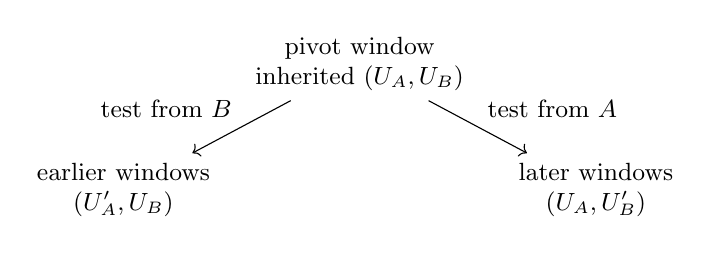
\begin{tikzpicture}[every node/.style={align=center,font=\small}]
 \node (pivot) at (0,0) {pivot window\\inherited \((U_A,U_B)\)};
 \node (left) at (-3,-1.6) {earlier windows\\\((U_A',U_B)\)};
 \node (right) at (3,-1.6) {later windows\\\((U_A,U_B')\)};
 \draw[->] (pivot) -- node[above left] {test from \(B\)} (left);
 \draw[->] (pivot) -- node[above right] {test from \(A\)} (right);
\end{tikzpicture}
\caption{A pivot restricts the first points to its left and
the second points to its right. Its own targets use both
new caps. This is exactly the time direction in
\eqref{comp:average-incidence} and
\eqref{comp:target-incidence}.}
\label{comp:tree-figure}
\end{figure}

All calls use fresh independent public tables. Their
acceptance predicates are exactly those prescribed in
Lemmas~\ref{geom:description} and \ref{geom:validation},
applied to the trimmed inputs \(S,T\) and the captured
subsets produced by those lemmas. These inputs are
determined by the original auxiliary supports, the
history and indices, and earlier auxiliary tables.
Conditional marginal laws are used to choose the original
supports, not as an additional acceptance filter.
No call inspects actual unexposed flags. Thus, given the
history and indices, the entire auxiliary construction
remains independent of those flags. In the loss estimates
below, we compare each test's hidden source with its
original pivot support, which still supplies the
unconditioned incidence bounds.

\begin{lemma}\label{comp:tree-loss}
The expected number of middle targets lost through the
pre-tree deletions, deleted subtrees, or exclusion by the
produced caps is \(o(k)\). In particular, a prescribed
deterministic number \(\Theta(k)\) of targets can be retained in order
with probability bounded below.
\end{lemma}

\begin{proof}
The pre-tree deletions have already been bounded, and all
windows have equal size. It remains to analyze the tests
without conditioning on the later retention of a window.

Fix the history, indices, all original support choices,
and any earlier auxiliary data making a validation test
ready. In the first validation test the hidden source is
the intersection of the described set with one trimmed
support. Description capture and the \(.9\) trim make it
a fixed positive fraction of the corresponding original
support. If this test succeeds, the second test's hidden
source is also a fixed positive fraction of its original
support, by the \(.99\) capture assertion of
Lemma~\ref{geom:validation}.
For either test and every fixed opposite point \(y\), let
\(E_y\) be the event that the test is produced and excludes
\(y\) by its ambient test.
Lemma~\ref{geom:produced-test} gives
\begin{equation}\label{comp:pointwise-test}
 \Prob(E_y\mid\text{readiness data})
       \le Cq\frac{|X\cap N(y)|}{|X|},
\end{equation}
where \(X\) is that test's original pivot support.
The right side no longer depends on the readiness data.
The contribution is zero if the node is not reached or
the test is not ready. We may consequently average over
all earlier auxiliary data with no additional conditioning.

More explicitly, fix one ancestor test and a descendant's
corresponding original support \(Y\). Let \(L\) be the
fraction of \(Y\) excluded by that test, set to zero when
the test is not produced. If \(\mathcal H\) denotes the
history and indices, and \(\mathcal S\) all original support
choices, averaging over readiness data gives
\[
 \E(L\mid\mathcal H,\mathcal S)
       \le Cq\frac{e(X,Y)}{|X||Y|}.
\]
This bound is not conditioned on reaching the test.
Now average the original support choices under their
original independent law.
The chronological inheritance rule ensures that the pair
is always an earlier first support against a later second
support. Equation~\eqref{comp:average-incidence} bounds the
expected lost fraction by \(C\varepsilon\) per ancestor
test. This remains true when readiness data or the
prescribed acceptance predicates depend on other original
support sets: those sets were fixed before
\eqref{comp:pointwise-test} was applied.

At a node of depth \(j\), failure of a trim after all
previous successes requires loss of at least one tenth
of an original support to its ancestor tests. The joint
probability of this event and reaching the node is
therefore at most \(Cj\varepsilon\).
By \eqref{comp:average-incidence} and Markov's inequality,
the unconditional same-node density rejection probability
is at most \(C\sigma^{-1000\beta}\).
Conditional on reaching a ready node, a description or
validation failure costs \(Ce^{-cq}\), uniformly in its
input data. Hence, if \(H=C\log(w+2)\), a fixed window's
probability of deletion somewhere along its path is at
most
\begin{equation}\label{comp:subtree-loss}
 C\varepsilon H^2+
 C\sigma^{-1000\beta}H+Ce^{-cq}H=o(1).
\end{equation}

For an actual good middle target, instead integrate
\eqref{comp:pointwise-test} against its unnormalized good
endpoint mass. Independence of the auxiliary construction
from actual unexposed flags and
\eqref{comp:target-incidence} give an exclusion probability
at most \(C\varepsilon\) per relevant ancestor test.
Both tests are relevant at the target's own pivot.
This count includes a first test as soon as it is
produced, even if the second test subsequently fails.
Neither this estimate nor \eqref{comp:subtree-loss}
conditions on eventual survival of a descendant or target.

The expected bad-index fraction tends to zero by
Proposition~\ref{mark:good-indices}, and the bad-endpoint
mass at every good index tends uniformly to zero by
Lemma~\ref{mark:endpoint-mass}.
Combining these losses with \eqref{comp:subtree-loss}
and the \(O(H)\) relevant tests gives expected total
loss \(o(k)\).
The original middle-target population is a fixed positive
multiple of \(k\). With probability tending to one,
at least a prescribed smaller positive multiple remains;
retain the first prescribed number in order.
\end{proof}

\subsection{The new decoder and its message length}

The loss argument has shown that many targets survive.
We must now verify that their domains can be reconstructed
from the new message alone, and that the message has the
bound asserted in Lemma~\ref{comp:step}.

The message specifies the surviving-list tree, construction
statuses, all successful node descriptions and validation
messages, the necessary support sizes and orientations,
and the number of retained targets at each pivot.
These additional discrete data cost \(O(w\sigma)\) bits.
In particular, original slot labels are not sent.
Traversing the tree in chronological order and using the
retained counts specifies the domain of each new tuple
slot.

The decoder starts with full point domains, prescribed
public parameters, and a fresh table address for every
call at every tree address. It reconstructs the domains
recursively from successful messages.
At each successful node its header supplies \(n_A,n_B\)
and the orientation and mode choices. The inherited domains
then determine \(d_A,d_B\). In particular, the validation
row lengths \(\lceil C_0q(d_A+1)\rceil\) and
\(\lceil C_0q(d_B+1)\rceil\), and the associated finite search
cutoffs, are determined from these data and public constants.
Any other row-length diagnostics required inside a
description are sent within that lemma's message budget.
Table addresses consist of the binary tree word, the call
phase (description, first validation, or second validation),
and the internal call address used by that subroutine.
Thus neither the table choice nor a variable row length
requires the old history.
An acceptance predicate can involve a hidden support,
but the accepted proposal row is recoverable from its
transmitted index without checking that predicate again.
A failed construction deletes its whole subtree; no
retained descendant depends on a failed test that was
not transmitted. This also explains why descriptions
of failed constructions need not be part of the message.
None of this reconstruction uses the old context,
conditional laws, or hidden support sets.

At a successful node, validation gives
\[
 |U_A'|\le Cq^{d+1}/n_B,\qquad
 |U_B'|\le Cq^{d+1}/n_A.
\]
Since \(n_An_B\ge q^{d+1}e^{-CK_*}\), mixing between
the two caps gives at most
\begin{equation}\label{comp:new-domain}
 Cq^d e^{CK_*}
\end{equation}
incident flags in their product. This is the domain
assigned to each retained target at that pivot.

An independent ambient-size bound at each node would charge
\(O(\sigma)\) at every pivot. Instead, the two children
jointly receive the parent's two marginal gaps, up to
\(O(K_*)\). We use this additive bound to sum the costs
level by level. Put
\[
 G=\log(|U_A||U_B|/q^{d+1})
\]
at a node with nonempty data. Its support gaps obey
\begin{equation}\label{comp:gap-potential}
 d_A+d_B\le G+CK_*.
\end{equation}
The description and validation together cost
\(O(qP(d_A+d_B+P))\).
For a successful node the children satisfy
\[
 G_{\rm left}^+\le d_B+C,\qquad
 G_{\rm right}^+\le d_A+C,
 \qquad x^+=\max(x,0).
\]
Indeed the left child inherits \(U_A',U_B\), so its
untruncated potential is at most
\(\log(C|U_B|/n_B)=d_B+C\); the other child is symmetric.
It follows from \eqref{comp:gap-potential} that
\begin{equation}\label{comp:potential-branch}
 G_{\rm left}^++G_{\rm right}^+
       \le G^++CK_*.
\end{equation}
The root potential is \(O(\sigma)\).
Pruning can only reduce a positive-potential sum, and
charging \eqref{comp:potential-branch} to the at most
\(w\) ancestors shows that the sum of positive
potentials at any level is at most
\(C(\sigma+wK_*)\).
There are \(O(\log(w+2))\) levels. Summing the successful
node costs, using \(K_*=o(P)\), and including the
additional discrete data gives the deterministic bound
\begin{equation}\label{comp:tree-cost}
 CqP\log(w+2)(\sigma+wP)+Cw\sigma.
\end{equation}
All row searches have the prescribed finite cutoffs of
the description and validation lemmas, so this is a
maximum message-length bound, not only an expected one.
Self-delimiting messages convert it to the same entropy
bound after an absolute constant adjustment.

\begin{proof}[Proof of Lemma~\ref{comp:step}]
Apply the preparation of Section~\ref{mark:section}.
Its class selection conditions on an event of probability
bounded below; its choices and orientation are determined
by the revealed history. In a high-rank class use
Lemma~\ref{comp:high-rank}, with \(w=1\).
Its cost \(O(q\sigma^{1+\beta})\) is bounded by
\eqref{comp:step-bounds}, and its exponent \(O(K)\)
is \(O(K_*)\).
In a reciprocal class use the support construction,
tree, and Lemma~\ref{comp:tree-loss}.
Equations~\eqref{comp:new-domain} and
\eqref{comp:tree-cost} give the required output budgets.
The window sizes in \eqref{mark:windows} imply
\[
 w\le C\sigma^{1+\eta/2}/D
\]
in both reciprocal cases, and this bound also holds
for \(w=1\) under the admissible range of \(D\).

Initially average over the fresh public tables as well
as the auxiliary support choices and other randomness.
The preceding arguments give a probability bounded
below of having the required number of targets and
all asserted output properties. Hence some fixed
choice of the entire public table family retains a
bounded-below probability of this event. Fix that
family first, then condition on successful extraction
of the prescribed deterministic length.
The fresh table family was independent of the input stream,
so fixing it does not change the input stream's marginal law.
For any stream event, the subsequent success conditioning increases its
probability by at most the reciprocal of the fixed
success probability. Thus constant domination
persists, while the occupancy property persists
pointwise. The retained tuple is an ordered subtuple
in the selected orientation and remains consistent.

The message-length and domain bounds hold for every
successful history and every fixed table realization,
not merely on average over histories. They therefore
remain valid under this possibly biased conditioning.
The new context is precisely its standalone message,
not that message together with the old history.
Consequently its entropy and slot domains satisfy
\eqref{comp:step-bounds}, with fixed constants, as
asserted.
\end{proof}

\section{Completion of the construction and the Ramsey bounds}
\label{end:section}

The preceding compression step replaces an old description by a new
one while retaining a fixed positive fraction of the selected tuple.
We now iterate that replacement a bounded number of times. The final
description has too little entropy to encode a selected tuple from the
original stream. We then pass from the resulting prime-indexed graphs
to every sufficiently large integer $t$ and prove the matching upper
estimate.

\subsection{A bounded number of compression stages}
\label{end:construction}

\begin{proof}[Proof of Theorem~\ref{intro:prime-construction}]
Fix $d\ge5$ and $0<\eta<1/10$, with all the parameters of
Equation~\eqref{base:stream-parameters}. Suppose, for a contradiction,
that every stream has a consistent $k$-tuple. Select one by a fixed
rule, and condition on the simultaneous rectangle event of
Lemma~\ref{base:rectangles}. For large $q$ this event has probability
at least $1/2$, so the new stream law is dominated by twice the iid
law. The selected tuple has deterministic length $k$.

Initially the context is empty. Its entropy budget is $\Lambda_0=0$,
and the full flag domain has size
\[
 Q_dQ_{d-1}\le4q^d\exp((d-1)\sigma).
\]
Thus we may take $\Delta_0=(d-1)\sigma$. The stage parameter defined
in Equation~\eqref{mark:parameters} is initially
\[
 D_0=\sigma^\beta\bigl(1+(d-1)\sigma^{1-\eta}\bigr)
     =O(\sigma^{1-\eta+\beta}),
\]
which lies in the admissible interval
$[\sigma^\beta,\sigma^{1-\eta/2}]$ for sufficiently large $q$.

Consider any admissible stage with budgets $\Lambda,\Delta$ and
parameter $D$. By Lemma~\ref{comp:step}, its replacement context has
budgets satisfying
\begin{equation}
 \Lambda'\le CqP\log(w+2)(\sigma+wP)+Cw\sigma,
 \qquad \Delta'\le CK_*,
 \qquad 1\le w\le C\sigma^{1+\eta/2}/D.
 \label{end:one-step-budget}
\end{equation}
The high-rank case is included with $w=1$. The constants may depend on
$d,\eta$, a fixed lower bound for $\ell/k$, and fixed upper bounds for
the stream domination factor and the domain prefactor. They are uniform
over all input laws, contexts, conditional histories, and class choices
satisfying those numerical bounds, as in Lemma~\ref{comp:step}.
Using $k\asymp q\sigma^{1+\eta}$ and
$P\le4D\sigma^{9\beta}$, the three terms to estimate satisfy
\[
 \frac{qP\sigma}{k}\le CD\sigma^{9\beta-\eta},\qquad
 \frac{qP^2w}{k}\le CD\sigma^{18\beta-\eta/2},\qquad
 \frac{w\sigma}{k}\le\frac{Cq^{-1}\sigma^{1-\eta/2}}{D}.
\]
Also $\log(w+2)=O(\log(\sigma+2))$. We obtain
\begin{align}
 \frac{\Lambda'}{k}
 &\le CD\log(\sigma+2)
       \bigl(\sigma^{9\beta-\eta}
                  +\sigma^{18\beta-\eta/2}\bigr)
       +\frac{Cw\sigma}{k}\notag\\
 &\le D\sigma^{-\eta/3}.
 \label{end:entropy-contraction}
\end{align}
Indeed, $w\sigma/k\le Cq^{-1}\sigma^{1-\eta/2}/D$ is exponentially
small in $\sigma$, uniformly for admissible $D$. The other two terms
have exponents strictly below $-\eta/3$, because
$\beta=\eta/10^7$; their fixed constants and logarithmic factor are
absorbed for large $q$.

Recompute the stage parameter from the new budgets, without retaining
the old context. Equations~\eqref{mark:parameters} and
\eqref{end:entropy-contraction} give
\begin{align}
 D_{\rm new}
 &=\sigma^\beta\bigl(1+\Lambda'/k+\Delta'\sigma^{-\eta}\bigr)
   \notag\\
 &\le\sigma^\beta
     +D\sigma^{\beta-\eta/3}+CD\sigma^{7\beta-\eta}
   \notag\\
 &\le\sigma^{2\beta}+D\sigma^{-\eta/4}.
 \label{end:parameter-contraction}
\end{align}
The last inequality follows from
$\beta-\eta/3<-\eta/4$ and $7\beta-\eta<-\eta/4$.
This recurrence preserves admissibility: its lower bound
$D_{\rm new}\ge\sigma^\beta$ follows from the definition, while
\[
 \sigma^{2\beta}+\sigma^{1-3\eta/4}
 \le\sigma^{1-\eta/2}
\]
for large $q$.

Choose the number of stages in advance, for example
$T=\lceil8/\eta\rceil$. Iterating
Equation~\eqref{end:parameter-contraction}, and using $D_0\le\sigma$
for large $q$, gives
\[
 D_T\le\sigma^{1-T\eta/4}
       +\frac{\sigma^{2\beta}}{1-\sigma^{-\eta/4}}
       \le2\sigma^{2\beta}.
\]
One further compression stage produces budgets $\Lambda_*,\Delta_*$
with
\begin{equation}
 \frac{\Lambda_*}{k}
     \le2\sigma^{2\beta-\eta/3}=o(1),
 \qquad
 \frac{\Delta_*q\sigma}{k}
     \le C\sigma^{8\beta-\eta}=o(1).
 \label{end:final-budgets}
\end{equation}

We justify explicitly the probabilistic invariants throughout this
iteration. At each stage Lemma~\ref{comp:step} first averages over
fresh public tables and fixes a table family with an extraction event
of probability bounded below. It then conditions on that event and
retains a prescribed deterministic number of slots in one of the two
allowed orientations. The new decoder uses only its new context and
its fixed tables. In particular, its entropy budget is $\Lambda'$,
not the sum of earlier context entropies. Every retained tuple is
consistent, remains in the original stream in an allowed orientation,
and still satisfies the simultaneous rectangle bound.

The constants and thresholds can be fixed without knowing the actual
conditional laws. Start with the numerical bounds $\ell/k=1$, domain
prefactor $4$, and domination factor $2$. The uniform statement of
Lemma~\ref{comp:step} supplies a positive lower bound on the next
retained proportion and on the conditioning probability, and an upper
bound on the next domain prefactor. Use these to prescribe the next
stage's numerical bounds, including the old domination bound divided
by the success-probability lower bound. Recursively do this for the
already fixed $T+1$ stages, taking maxima over the finitely many class
types if necessary. All resulting constants are independent of $q$;
choose $q$ above their finitely many uniform thresholds and the
arithmetic thresholds used above. No enumeration of conditional
histories, or history-dependent limiting argument, is involved.

Consequently the final length is deterministic and satisfies
$\ell_*=\Theta(k)$, and the final stream law still has a constant
domination factor. Lemma~\ref{base:selection-entropy} therefore
applies to the final tuple $F_*$. Only the marking scans are now
performed: no further class selection, tuple extraction, or
conditioning is used. The marking message specifies the expensive
flag values and a cheap domain for each remaining slot. Conditional
on that message, the entropy of the remaining values is bounded by
the logarithm of the product of those domains. Thus
Equation~\eqref{mark:entropy-upper} bounds the entropy of the entire
tuple under its present law.

Therefore, Equation~\eqref{mark:entropy-upper} from the final
marking scan and Equation~\eqref{end:final-budgets} give
\[
 H(F_*)\le d\sigma\ell_*+\Lambda_*+O(k)+O(\Delta_*q\sigma)
          =d\sigma\ell_*+O(k).
\]
Lemma~\ref{base:selection-entropy} gives instead
\[
 H(F_*)\ge d\sigma\ell_*+\eta\ell_*\log\sigma-O(k).
\]
These inequalities contradict each other, since
$\ell_*\ge c k$ for a fixed $c>0$ and $\log\sigma\to\infty$.
Consequently some stream has no consistent $k$-tuple. Its flag graph
has independence number less than $k$ and is $K_{d+1}$-free by
Lemma~\ref{base:flag-graph}, as required.
\end{proof}

\subsection{From prime orders to every integer}

Only a fixed-ratio interval between consecutive available prime scales
is needed. We include an elementary proof to avoid imposing a
prime-subsequence restriction on the Ramsey bound.

\begin{lemma}[A prime in a fixed-ratio interval]
\label{end:prime-interval}
There is a constant $c_0>0$ such that, for every sufficiently large real
$x$, a prime $q$ satisfies $c_0x\le q\le x$.
\end{lemma}

\begin{proof}
Define
\[
 \vartheta(x)=\sum_{p\le x}\log p,
 \qquad
 \psi(x)=\sum_{\substack{p^h\le x\\h\ge1}}\log p,
\]
where $p$ ranges over primes. Every prime in $(m,2m]$ divides
$\binom{2m}{m}$, so
\[
 \vartheta(2m)-\vartheta(m)
 \le\log\binom{2m}{m}\le2m\log2.
\]
Summing at powers of two and then using monotonicity proves
$\vartheta(x)\le Cx$.

The exponent of $p$ in the central binomial coefficient is
\[
 \sum_{h\ge1}
 \left(\left\lfloor\frac{2m}{p^h}\right\rfloor
        -2\left\lfloor\frac{m}{p^h}\right\rfloor\right).
\]
Each summand is zero or one, and therefore
\[
 \psi(2m)\ge\log\binom{2m}{m}
 \ge2m\log2-\log(2m+1).
\]
The last inequality follows because the largest of the $2m+1$
binomial coefficients is at least their average $4^m/(2m+1)$.
For proper prime powers the rough estimate
\[
 0\le\psi(x)-\vartheta(x)
   \le C\sqrt{x}\log^2(x+2)=o(x)
\]
suffices: there are $O(\log x)$ exponents $h\ge2$, at most
$\sqrt{x}$ possible bases for each, and each weight is at most
$\log x$. It follows first for even integers, and then by monotonicity
for all large real $x$, that $\vartheta(x)\ge cx$.
Choose $c_0<c/(2C)$. For sufficiently large $x$,
$\vartheta(x)>\vartheta(c_0x)$, proving that the stated interval
contains a prime.
\end{proof}

Fix $s\ge6$, put $d=s-1$, and choose $0<\eta<1/10$.
For a sufficiently large integer $t$, apply
Lemma~\ref{end:prime-interval} with
\[
 x=\frac{t}{(\log t)^{1+\eta}}.
\]
The resulting prime tends to infinity, and $\log q\sim\log t$.
Moreover,
\[
 q(\log q)^{1+\eta}
 \le t\left(\frac{\log q}{\log t}\right)^{1+\eta}<t.
\]
The graph from Theorem~\ref{intro:prime-construction} therefore has no
independent set of size $t$. Its order gives
\begin{equation}
 r(s,t)>\lfloor q^d\log q\rfloor
 \ge c_{s,\eta}\frac{t^d}{(\log t)^{d-1+d\eta}}.
 \label{end:lower-slack}
\end{equation}
Here the floor is absorbed into a fixed positive constant for large
$t$. Given any $\varepsilon>0$, choose
$\eta=\min\{1/20,\varepsilon/(2d)\}$. Then
$\varepsilon-d\eta>0$, so
$(\log t)^{\varepsilon-d\eta}$ eventually absorbs
$1/c_{s,\eta}$. Equation~\eqref{end:lower-slack} yields the required
coefficient-one lower bound for every sufficiently large integer $t$.

\subsection{The matching upper bound}

The upper estimate of Ajtai, Koml\'os, and Szemer\'edi \cite{AKS1980}
can be obtained from a triangle-free independence bound followed by
sampling and deletion. Shearer proved a lower bound asymptotic to
$n\log d/d$ as $d\to\infty$ for triangle-free graphs of average degree $d$
\cite{Shearer1983}. The elementary proof below uses a uniformly chosen
independent set, following Alon's method
\cite[proof of Proposition~2.1]{Alon1996}; sharper
occupancy estimates appear in Davies, Jenssen, Perkins, and Roberts
\cite[Theorems~1 and~3]{DJPR2018}. We retain a convenient constant and give the details
separately from the lower-bound construction.

\begin{lemma}[Independent sets in a triangle-free graph]
\label{end:triangle-free}
If a triangle-free graph $H$ has $n>0$ vertices and maximum degree at
most a real number $D_0\ge1$, then
\[
 \alpha(H)\ge\frac{n\log(D_0+1)}{8(D_0+1)}.
\]
\end{lemma}

\begin{proof}
Choose an independent set $I$ uniformly from all independent sets of
$H$, including the empty set, and write $\mu=\E|I|/n$.
At a vertex $x$, expose $I$ outside the closed neighborhood of $x$.
Let $Z_x$ be the number of neighbors that have no neighbor in this
exposed part of $I$. These available neighbors are mutually
nonadjacent because $H$ is triangle-free. The remaining independent-set
choices are therefore $\{x\}$ or an arbitrary subset of the $Z_x$
available neighbors, all with equal conditional probability. Hence
\[
 \Prob(x\in I\mid\text{exposure})=\frac1{1+2^{Z_x}},
 \qquad
 \E(|I\cap N(x)|\mid\text{exposure})
   =\frac{Z_x2^{Z_x-1}}{1+2^{Z_x}}\ge\frac{Z_x}{4}.
\]
The last inequality includes $Z_x=0$.
Averaging also over a uniform vertex $x$, the degree bound gives
\[
 \frac{\E Z_x}{4}
 \le\frac1n\E\sum_{v\in I}\deg(v)\le D_0\mu.
\]
Since $(1+2^z)^{-1}\ge2^{-z}/2$ for $z\ge0$, Jensen's inequality
now gives
\begin{equation}
 \mu\ge\tfrac12\E 2^{-Z_x}
       \ge\tfrac12 2^{-\E Z_x}
       \ge\tfrac12 2^{-4D_0\mu}.
 \label{end:triangle-jensen}
\end{equation}
If $\mu<\log(D_0+1)/(8(D_0+1))$, then
Equation~\eqref{end:triangle-jensen} implies
$\mu>1/(2\sqrt{D_0+1})$, using $\log2<1$.
This is impossible: $\log u\le2\sqrt u$ for $u\ge1$ implies
$\log u/(8u)<1/(2\sqrt u)$. Thus $\mu$ has the claimed lower
bound, and $\alpha(H)\ge\E|I|=n\mu$ completes the proof.
\end{proof}

\begin{proposition}[Upper Ramsey estimate]
\label{end:upper-bound}
For every fixed integer $s\ge2$ there is a constant $C_s$ such that
for all sufficiently large integers $t$,
\[
 r(s,t)\le C_s\frac{t^{s-1}}{(\log t)^{s-2}}.
\]
\end{proposition}

\begin{proof}
Induct on $s$. The case $s=2$ follows from $r(2,t)=t$.
If a triangle-free graph has no independent set of size $t$, then all
its degrees are below $t$, because every neighborhood is independent.
Lemma~\ref{end:triangle-free}, with $D_0=t$, bounds its order by
$8t(t+1)/\log(t+1)$. This proves the case $s=3$.

Now let $s\ge4$ and suppose the estimate holds for smaller clique
parameters. Let $G$ have $n>0$ vertices, maximum degree $h$, no $K_s$,
and no independent set of size $t$. Every neighborhood avoids
$K_{s-1}$ and an independent $t$-set. Likewise the common neighborhood
of the two endpoints of an edge avoids $K_{s-2}$ and an independent
$t$-set. Therefore
\[
 h<r(s-1,t),\qquad
 |N(u)\cap N(v)|\le m:=r(s-2,t)\quad(uv\in E(G)).
\]
Summing these common-neighborhood sizes over edges counts each
triangle three times, so $G$ has at most $nhm/6$ triangles.

If $h\le t^{s-5/2}$, the greedy bound
$\alpha(G)\ge n/(h+1)$ gives
\[
 n<t(h+1)=O(t^{s-3/2})
   =o\!\left(\frac{t^{s-1}}{(\log t)^{s-2}}\right).
\]
Assume henceforth that $h>t^{s-5/2}$, and set
$\lambda=(hm)^{-1/2}\le1$. By the induction bound on $m$,
\begin{equation}
 \lambda h=\sqrt{h/m}
 \ge c_s t^{1/4}(\log t)^{(s-4)/2}\ge t^{1/5}
 \label{end:sample-degree}
\end{equation}
for sufficiently large $t$.

Retain each vertex independently with probability $\lambda$.
Delete all retained vertices whose degree in the sampled graph exceeds
$12\lambda h$, and then delete one vertex from each triangle still
present until none remains. If $E_0,T_0$ are the initial sampled edge
and triangle counts, respectively, the first deletion removes at most
$2E_0/(12\lambda h)$ vertices, and the second at most $T_0$.
Their expected numbers are at most
\[
 \frac{\lambda^2nh}{12\lambda h}=\frac{n\lambda}{12},
 \qquad
 \frac{\lambda^3nhm}{6}=\frac{n\lambda}{6}.
\]
Some realization therefore leaves a triangle-free induced subgraph
$H$ with
\[
 |V(H)|\ge\tfrac34n\lambda,
 \qquad \Delta(H)\le12\lambda h.
\]
Deleting further vertices cannot increase degrees, so both conclusions
hold simultaneously.
Lemma~\ref{end:triangle-free} and
Equation~\eqref{end:sample-degree} imply
\[
 t>\alpha(H)
 \ge\frac{(3/4)n\lambda\log(12\lambda h+1)}{8(12\lambda h+1)}
 \ge c\frac{n\log t}{h}.
\]
Finally substitute $h<r(s-1,t)$ and its induction bound to obtain
$n\le C_s t^{s-1}/(\log t)^{s-2}$. Increasing $C_s$ absorbs the
additive one in passing from the order of an avoiding graph to its
Ramsey number.
\end{proof}

\subsection{The logarithmic exponent}
\label{end:main-proof}

\begin{proof}[Proof of Theorem~\ref{intro:main}]
The lower bound follows from Equation~\eqref{end:lower-slack} and the
choice of $\eta$ made there. Proposition~\ref{end:upper-bound} gives
the asserted upper estimate. For every fixed $\varepsilon>0$, its
constant is eventually bounded by $(\log t)^\varepsilon$; hence
\[
 \frac{t^{s-1}}{(\log t)^{s-2+\varepsilon}}
 \le r(s,t)\le
 \frac{t^{s-1}}{(\log t)^{s-2-\varepsilon}}
\]
for all sufficiently large integer $t$. Taking logarithms and dividing
by $\log\log t>0$ bounds the expression in the theorem between
$s-2-\varepsilon$ and $s-2+\varepsilon$. Since $\varepsilon$ is
arbitrary, its limit is $s-2$.
\end{proof}

\bibliographystyle{plain}
\AddToHook{cmd/thebibliography/after}{\setlength{\itemsep}{2pt}}
\bibliography{references}

\end{document}
